% -------------------------------------------------------------------------
% RESULTADOS Y DISCUSION
% Este archivo esta pensado para incluirse dentro del capitulo de resultados.
% No contiene el comando \chapter (el capítulo se abre desde ejemplo-memoria.tex);
% la estructura interna usa \section para cada arquitectura y \subsection para sus apartados.
% -------------------------------------------------------------------------

% -------------------------------------------------------------------------
% RESULTADOS RESNET50
% -------------------------------------------------------------------------

\section{ResNet50}
\label{subsec:resultados_resnet50}

La arquitectura convolucional \textit{ResNet50} se utilizó como referencia frente a los modelos basados en transformers.

\subsection{Rendimiento por vista: estabilidad multi-semilla y checkpoint fijado}

La Figura~\ref{fig:multiseed_resnet50} resume la distribución del AUC de validación de ResNet50 a lo largo de las diez semillas, para cada plano anatómico.

\begin{figure}[H]
\centering
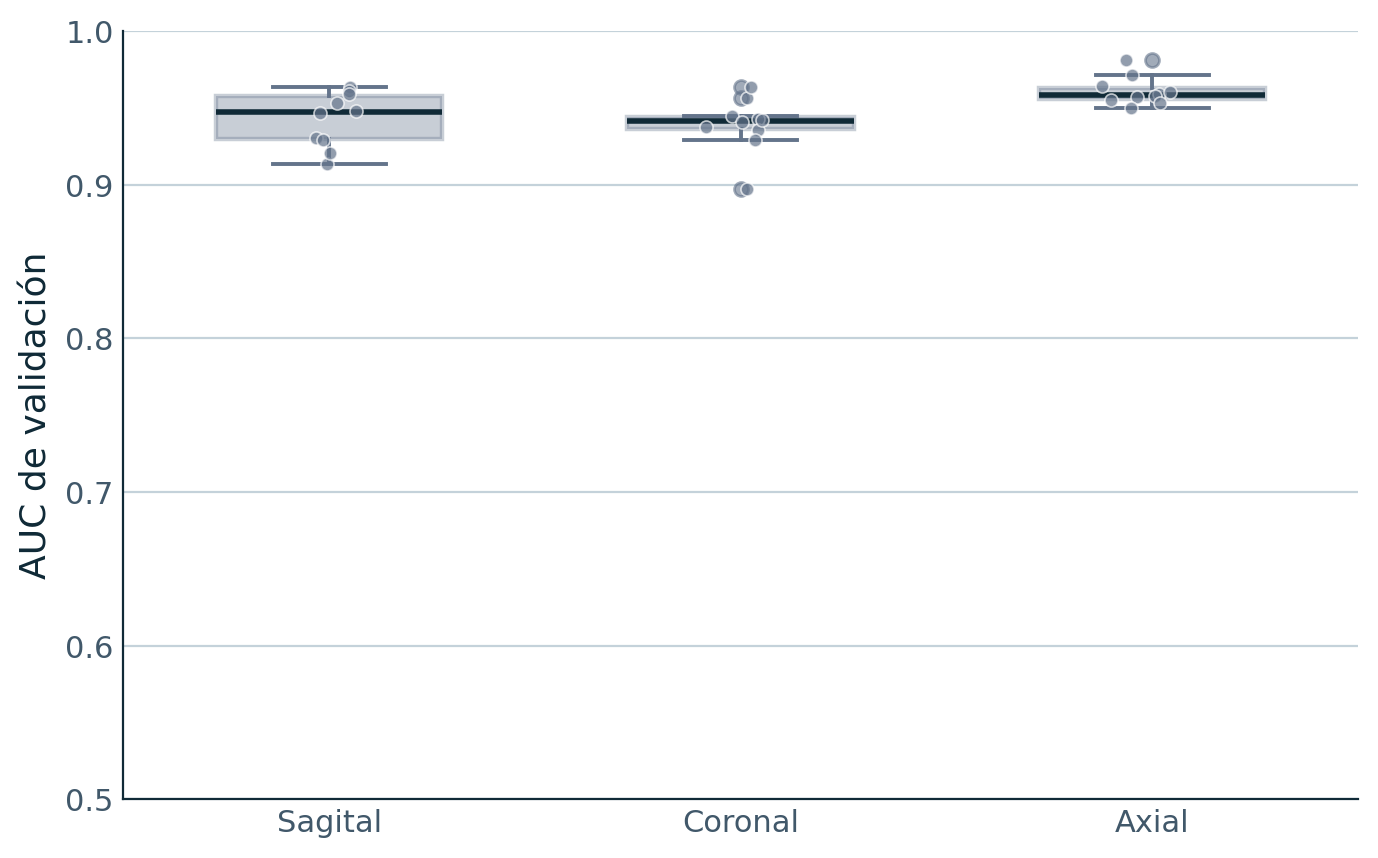
\includegraphics[width=0.82\textwidth]{figs/outputs/CNN_boxplot.png}
\caption{Distribución del AUC de \textbf{validación} de ResNet50 sobre las diez semillas (42--51) en cada plano anatómico. Cada punto corresponde a una semilla; la caja representa el rango intercuartílico y la línea central, la mediana.}
\label{fig:multiseed_resnet50}
\end{figure}

El plano axial presentó simultáneamente el mayor AUC medio (0.9610) y la menor dispersión entre semillas (desviación estándar de 0.0087), lo que se traduce en una caja estrecha y un comportamiento particularmente estable. Los planos sagital y coronal también mostraron valores medios elevados (0.9425 y 0.9390), aunque con una variabilidad notablemente mayor entre ejecuciones, visible en la mayor extensión de sus cajas. Esta diferencia refuerza la utilidad del análisis multi-semilla: una única ejecución podría sobreestimar o subestimar el rendimiento real de la arquitectura.

La Figura~\ref{fig:resnet_multiseed_training} muestra la evolución del entrenamiento multi-semilla de ResNet50 en los tres planos anatómicos.

\begin{figure}[H]
\centering
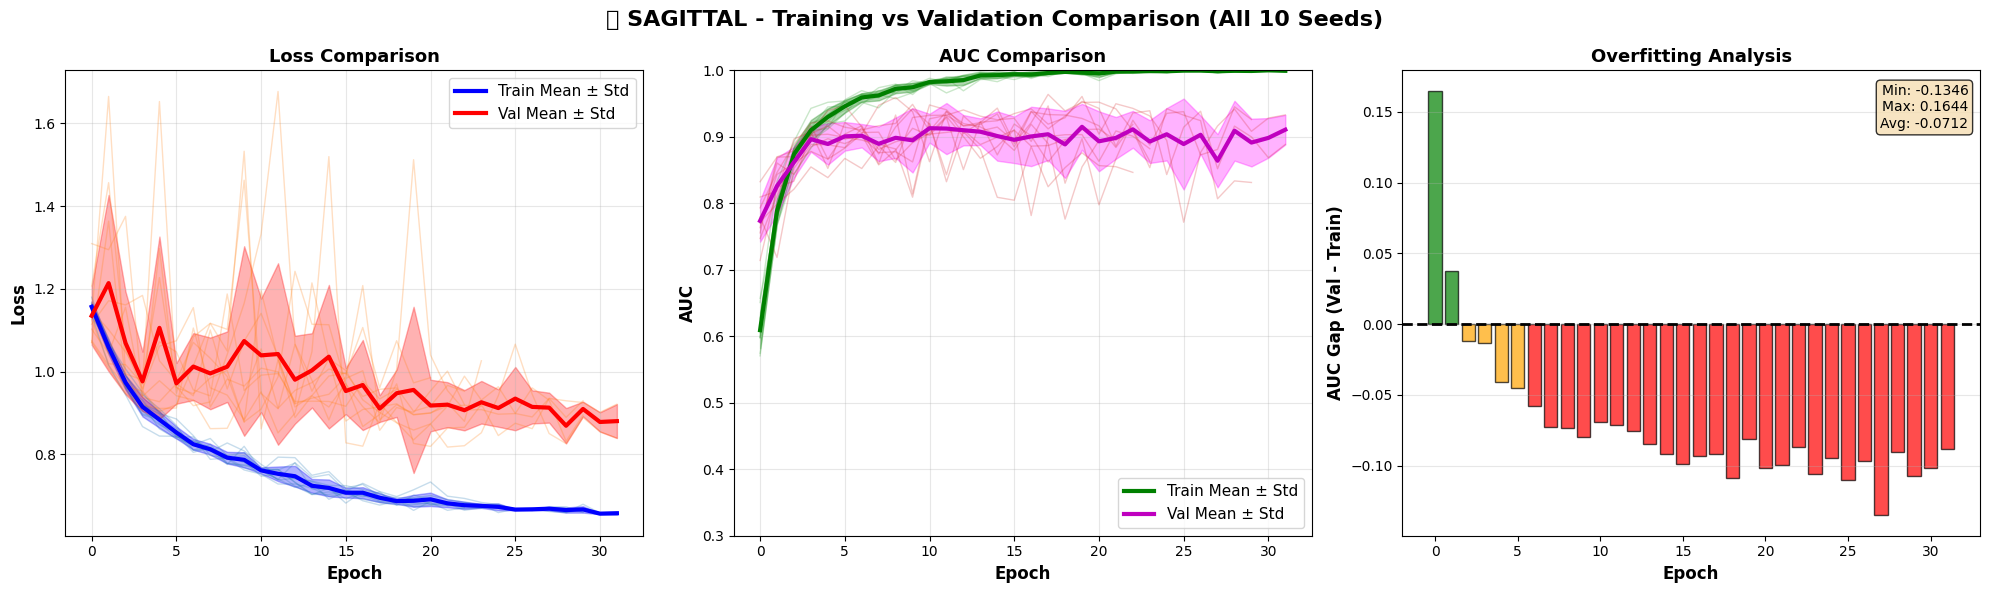
\includegraphics[width=0.88\textwidth]{figs/outputs/CNN_sagittal_entrenamiento_multiseed.png}

\vspace{0.6em}

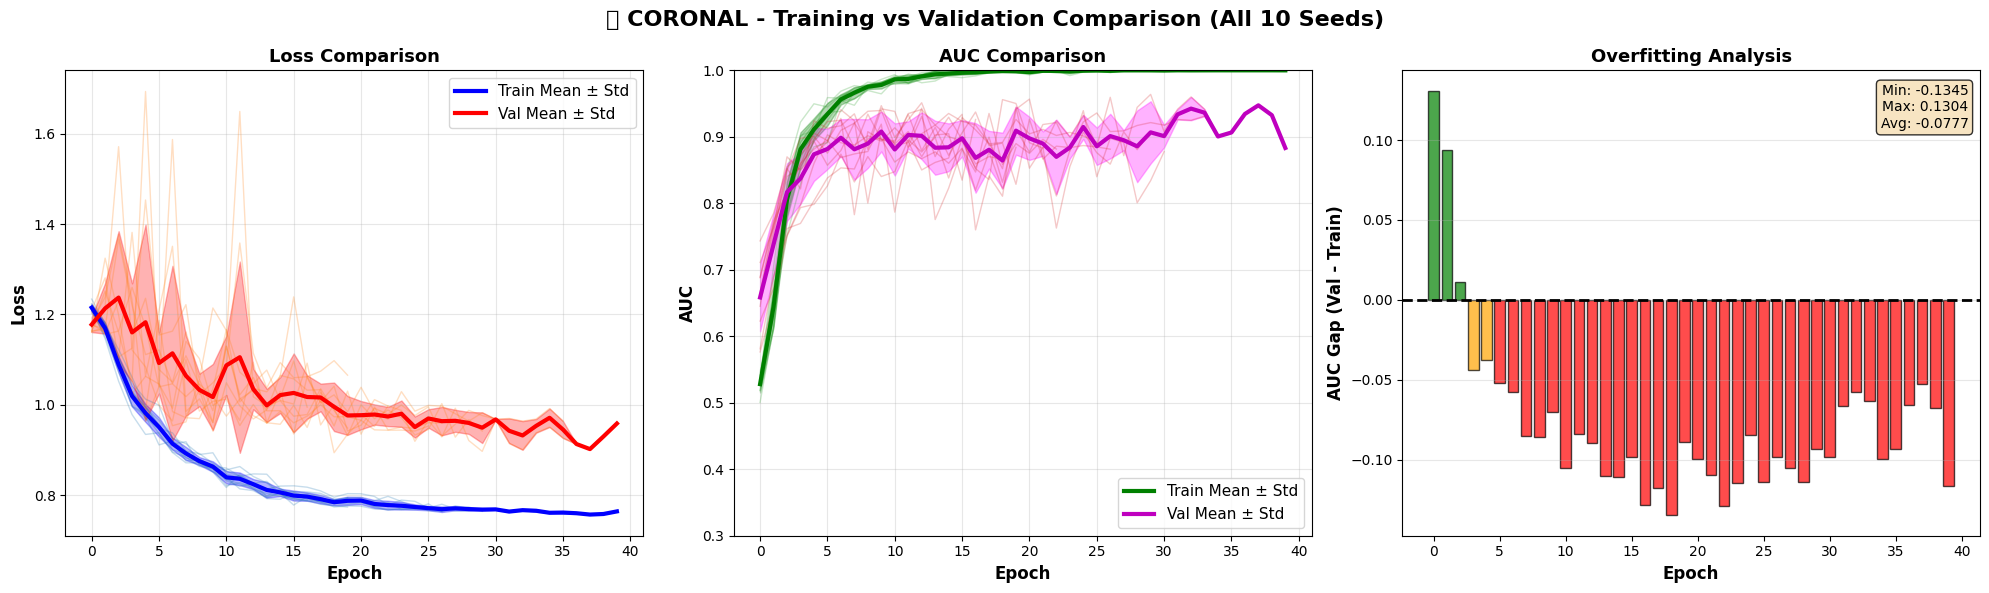
\includegraphics[width=0.88\textwidth]{figs/outputs/CNN_coronal_entrenamiento_multiseed.png}

\vspace{0.6em}

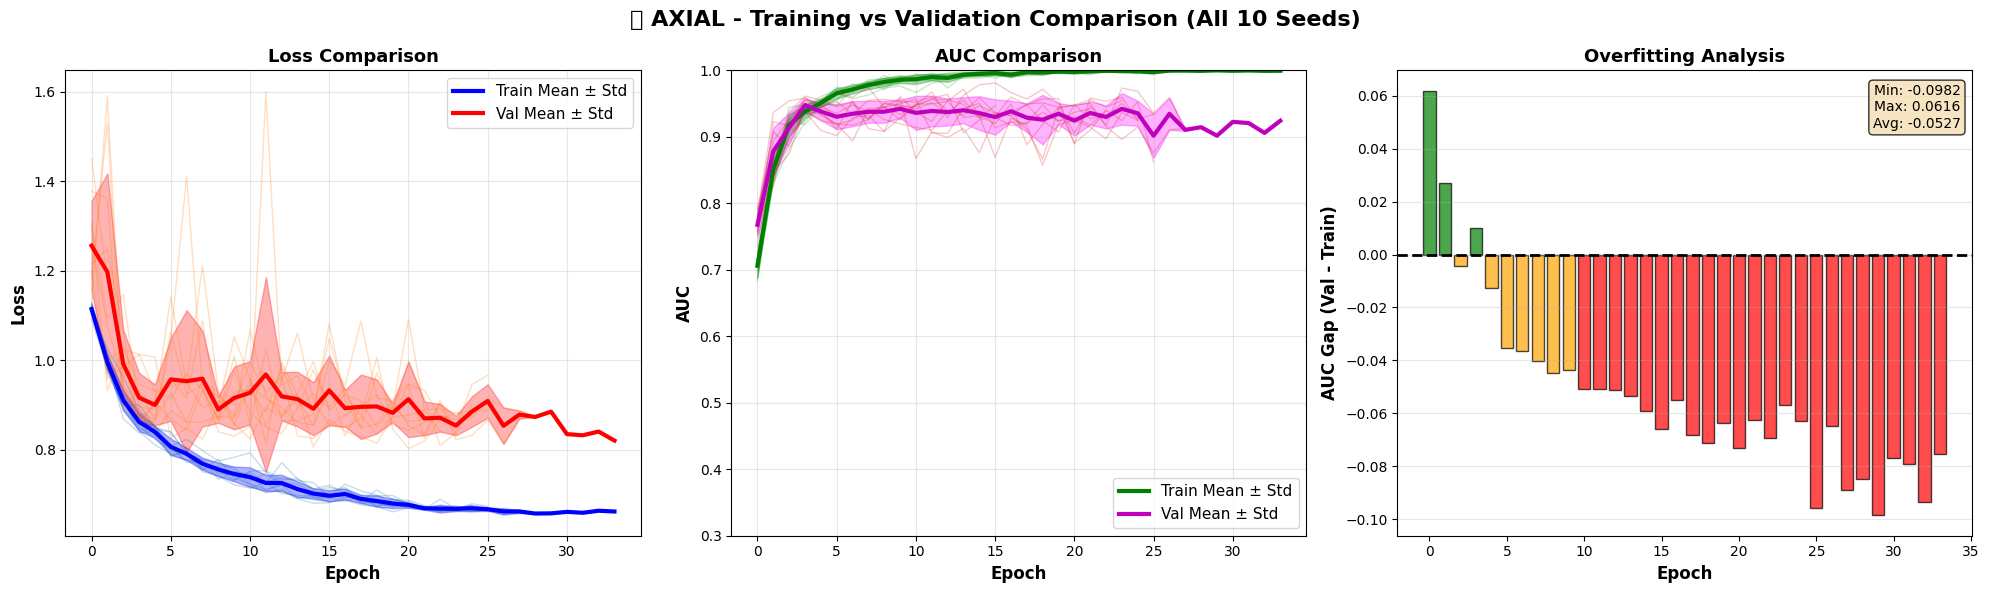
\includegraphics[width=0.88\textwidth]{figs/outputs/CNN_axial_entrenamiento_multiseed.png}
\caption{Evolución del entrenamiento multi-semilla de ResNet50 en los planos sagital, coronal y axial. Cada figura recoge, de izquierda a derecha, la pérdida de entrenamiento y de validación, el AUC de entrenamiento y de validación, y el análisis de sobreajuste ---la brecha de AUC entre validación y entrenamiento (Val $-$ Train) en cada época---; las curvas representan la media $\pm$ desviación típica de las diez semillas.}
\label{fig:resnet_multiseed_training}
\end{figure}

En estas curvas, la pérdida de entrenamiento desciende de forma sostenida mientras que la de validación se estabiliza y comienza a repuntar ligeramente a partir de aproximadamente la décima época, abriendo una brecha entre ambas que es la firma característica del sobreajuste. Este comportamiento justifica la estrategia de selección por \textit{early stopping} implícito: en lugar de conservar el último estado del modelo, se fija como checkpoint el de mejor AUC de validación, anterior al punto en que la brecha se ensancha. El tercer panel de cada figura (\textit{Overfitting Analysis}) cuantifica este efecto época a época mediante la brecha de AUC entre validación y entrenamiento (Val $-$ Train), promediada sobre las diez semillas. Cada barra corresponde a una época y su color resume la severidad: \textbf{verde} cuando la brecha es positiva o nula (la validación iguala o supera al entrenamiento, sin sobreajuste), \textbf{naranja} cuando es ligeramente negativa (entre $-0{,}05$ y $0$) y \textbf{roja} cuando cae por debajo de $-0{,}05$ (sobreajuste apreciable); la anotación del panel recoge los valores mínimo, máximo y medio de esa brecha a lo largo del entrenamiento. La lectura es directa: una brecha próxima a cero indica ausencia de sobreajuste, mientras que valores cada vez más negativos reflejan que el modelo ajusta mejor el conjunto de entrenamiento que el de validación. En las tres arquitecturas la brecha media se mantiene en el orden de unas pocas centésimas de AUC, lo que confirma un sobreajuste contenido y refuerza la validez de fijar el \textit{checkpoint} en el máximo de AUC de validación. La dispersión entre semillas es coherente con lo observado en el boxplot, siendo más acusada en los planos sagital y coronal que en el axial.

% (fusionado en Rendimiento por vista)

Tras el análisis multi-semilla, se fijó un checkpoint por plano anatómico utilizando únicamente el comportamiento observado en validación. El conjunto de test se empleó después solo como evaluación final. Estos resultados se resumen en la Tabla~\ref{tab:resnet_individual}.

\begin{table}[H]
\centering
\small
\caption{Rendimiento de los modelos ResNet50 fijados por plano anatómico utilizando únicamente validación.}
\label{tab:resnet_individual}
\begin{tabularx}{\textwidth}{
>{\raggedright\arraybackslash}X
>{\centering\arraybackslash}m{2.2cm}
>{\centering\arraybackslash}m{2.2cm}
}
\toprule
\textbf{Plano anatómico} &
\textbf{AUC validación} &
\textbf{AUC test} \\
\midrule
Sagital & 0.9501 & 0.8679 \\
Coronal & 0.9735 & 0.9246 \\
Axial   & 0.9704 & 0.9294 \\
\bottomrule
\end{tabularx}
\end{table}

En la evaluación final sobre test, el plano sagital obtuvo el menor rendimiento individual, mientras que el axial alcanzó el mayor AUC.

La Figura~\ref{fig:resnet_best_training} recoge las curvas de entrenamiento de los checkpoints finalmente fijados por validación para cada plano.

\begin{figure}[H]
\centering
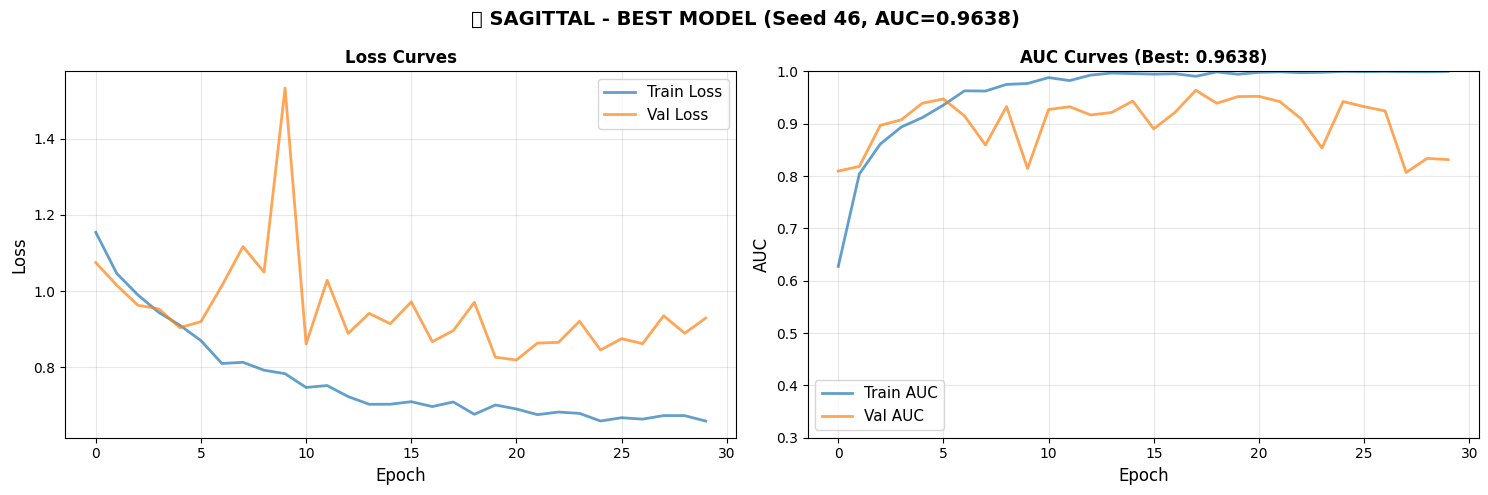
\includegraphics[width=0.88\textwidth]{figs/outputs/CNN_sagittal_best.png}

\vspace{0.6em}

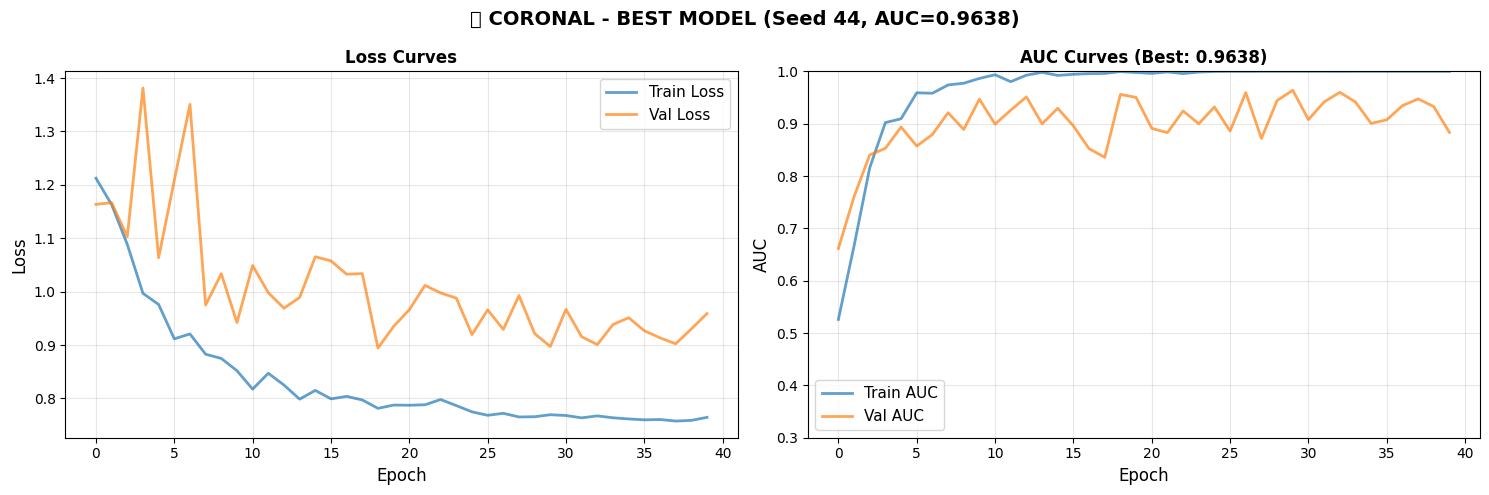
\includegraphics[width=0.88\textwidth]{figs/outputs/CNN_coronal_best.png}

\vspace{0.6em}

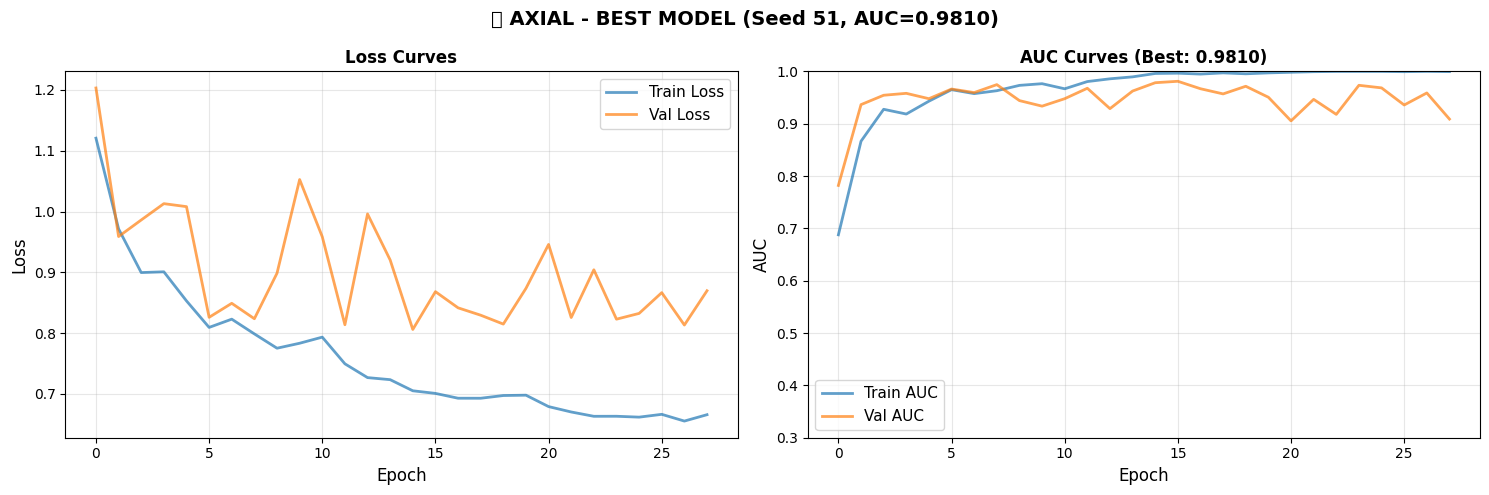
\includegraphics[width=0.88\textwidth]{figs/outputs/CNN_axial_best.png}
\caption{Curvas de entrenamiento de los mejores checkpoints de ResNet50 por plano anatómico.}
\label{fig:resnet_best_training}
\end{figure}

\subsection{Ensamble multi-vista calibrado}

El ensamble ResNet50 utilizó un umbral calibrado en validación de $\tau = 0.5445$. Sus métricas principales se recogen en la Tabla~\ref{tab:ensemble_resnet50_metricas}.

\begin{table}[H]
\centering
\scriptsize
\caption{Rendimiento del ensamble multi-vista basado en ResNet50 con umbral calibrado en validación (resultados en validación y test).}
\label{tab:ensemble_resnet50_metricas}
\begin{tabularx}{\textwidth}{
>{\raggedright\arraybackslash}X
>{\centering\arraybackslash}m{1.15cm}
>{\centering\arraybackslash}m{1.15cm}
>{\centering\arraybackslash}m{1.15cm}
>{\centering\arraybackslash}m{1.15cm}
>{\centering\arraybackslash}m{1.15cm}
>{\centering\arraybackslash}m{1.15cm}
>{\centering\arraybackslash}m{1.15cm}
}
\toprule
\textbf{Conjunto} &
\textbf{AUC} &
\textbf{Acc} &
\textbf{Prec.} &
\textbf{Recall} &
\textbf{Esp.} &
\textbf{F1} &
\textbf{Umbral} \\
\midrule
Validación & 0.9836 & 0.9362 & 0.7609 & 0.9722 & 0.9276 & 0.8537 & 0.5445 \\
Test       & 0.9545 & 0.8556 & 0.6333 & 0.8837 & 0.8472 & 0.7379 & 0.5445 \\
\bottomrule
\end{tabularx}
\end{table}

\begin{figure}[H]
\centering
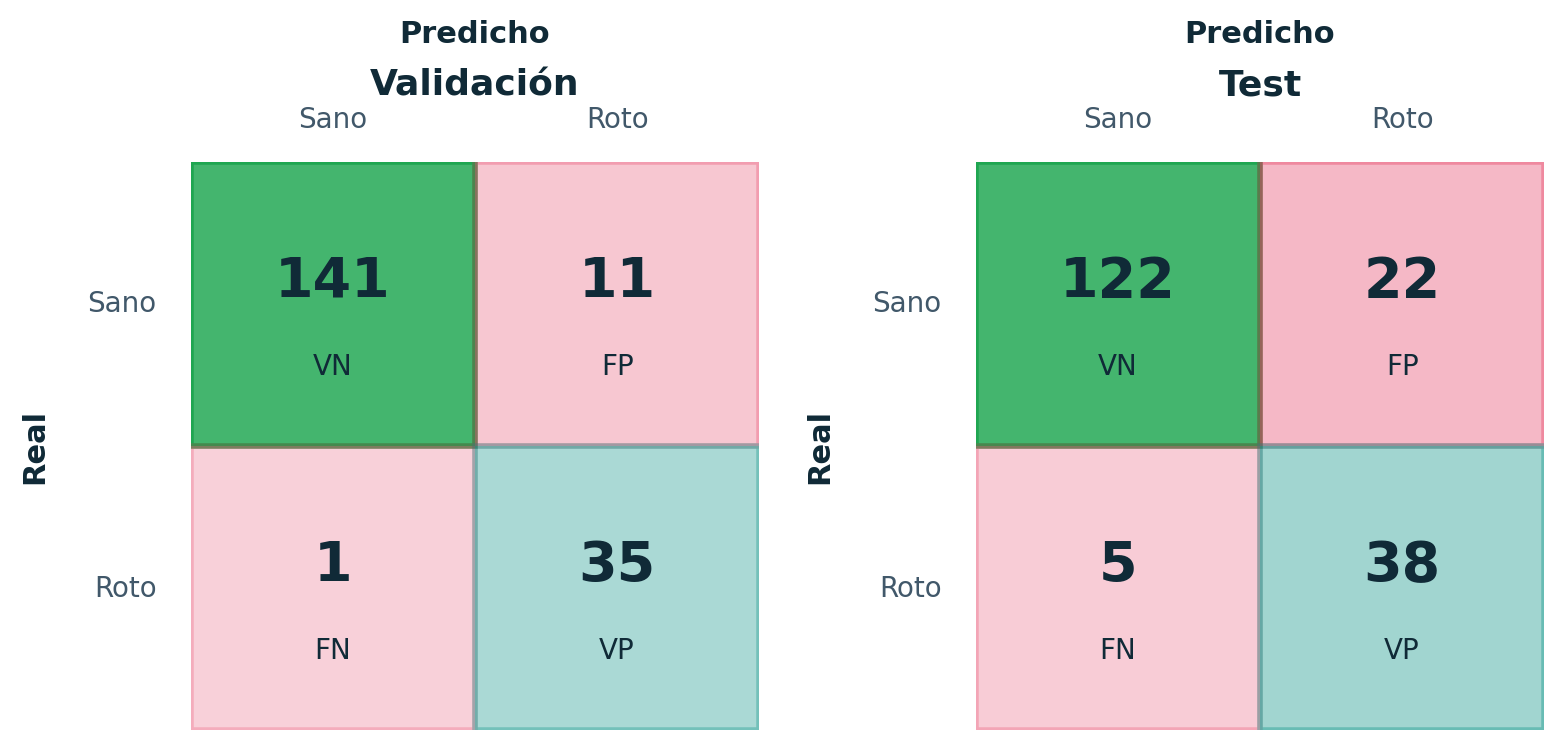
\includegraphics[width=0.92\textwidth]{figs/outputs/CNN_cm_grafica.png}
\caption{Matrices de confusión del ensamble ResNet50 en validación (izquierda) y test (derecha), con el umbral clínico fijado en validación.}
\label{fig:ensemble_resnet50_confusion}
\end{figure}

En la evaluación final sobre test de MRNet, el ensamble ResNet50 alcanzó un AUC de 0.9545. Su sensibilidad fue de 0.8837 (38 de las 43 roturas detectadas, 5 falsos negativos). La comparación entre las tres arquitecturas se aborda en la Sección~\ref{sec:comparativa_analisis}.

% -------------------------------------------------------------------------
% RESULTADOS VIT-SMALL
% -------------------------------------------------------------------------

\section{ViT-Small}
\label{subsec:resultados_vitbase}

\textit{Vision Transformer Small} (ViT-Small) procesa la imagen como una secuencia de parches y emplea autoatención global, con una dimensión de \textit{embedding} de 384 y aproximadamente 22 millones de parámetros. Se adopta como representante de la familia de transformers globales por su mejor equilibrio entre rendimiento y coste; la comparación con la variante mayor ViT-Base se aborda específicamente en la Sección~\ref{subsec:efecto_tamano}.

\subsection{Rendimiento por vista: estabilidad multi-semilla y checkpoint fijado}

La Figura~\ref{fig:multiseed_vitbase} presenta la distribución del AUC de validación de ViT-Small a lo largo de las diez semillas, para cada plano anatómico.

\begin{figure}[H]
\centering
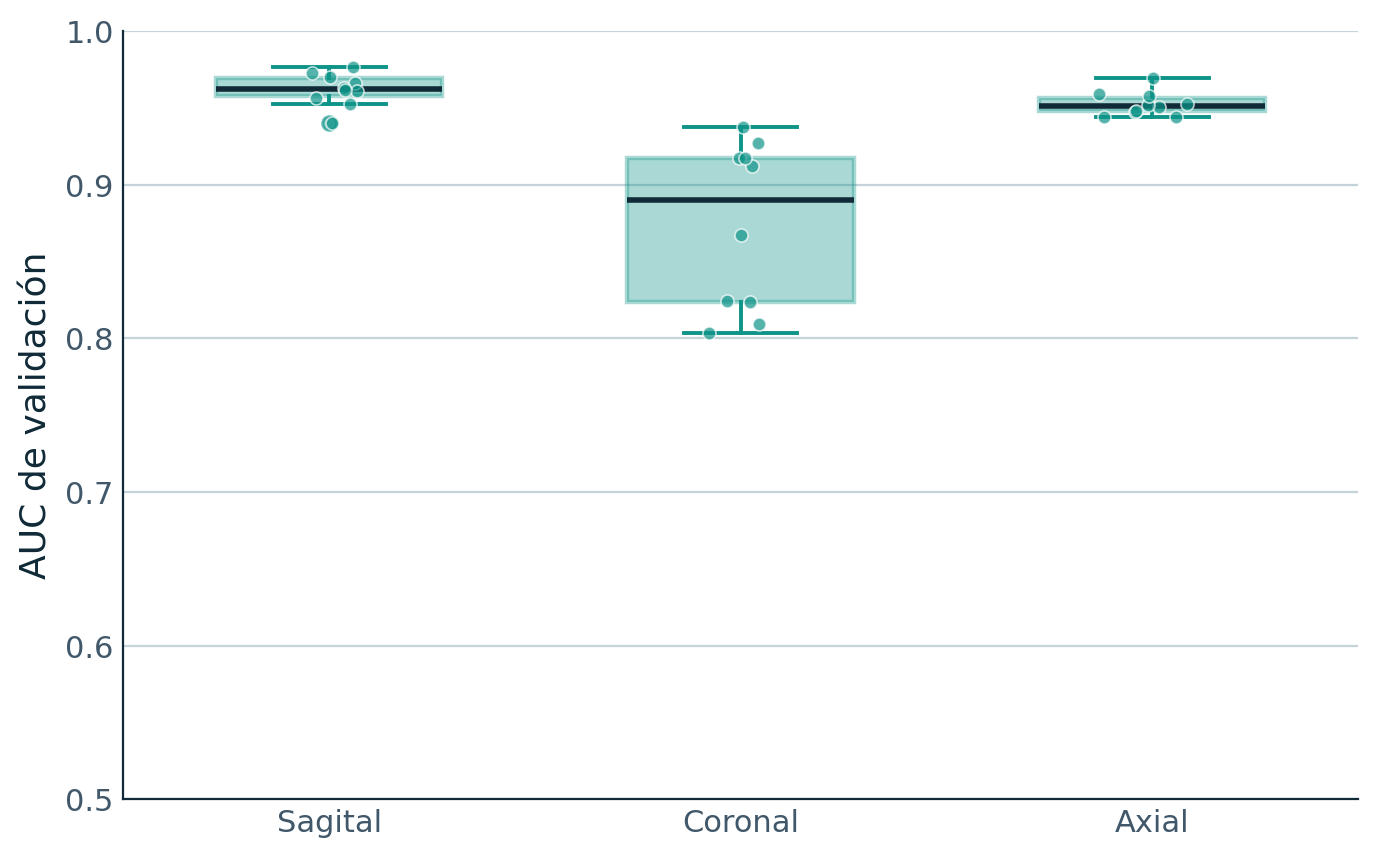
\includegraphics[width=0.82\textwidth]{figs/outputs/VIT_boxplot.png}
\caption{Distribución del AUC de \textbf{validación} de ViT-Small sobre las diez semillas (42--51) en cada plano anatómico. Cada punto corresponde a una semilla; la caja representa el rango intercuartílico y la línea central, la mediana.}
\label{fig:multiseed_vitbase}
\end{figure}

El análisis multi-semilla evidencia una diferencia importante entre planos. Los planos axial y sagital fueron los más estables, con desviaciones estándar de 0.0074 y 0.0100 respectivamente, mientras que el plano coronal presentó una variabilidad superior (0.0512). Esta inestabilidad puede explicarse por la dificultad de localizar de forma consistente el LCA en dicha proyección, donde la estructura puede aparecer parcialmente representada y con mayor interferencia de tejidos circundantes. Aun así, esta variabilidad es notablemente menor que la observada en otras arquitecturas para el mismo plano.

La sensibilidad de ViT-Small a la inicialización es coherente con la naturaleza de los transformers globales. Al no incorporar de forma explícita el sesgo inductivo de localidad espacial característico de las redes convolucionales, el modelo debe aprender durante el entrenamiento qué relaciones entre parches son relevantes. Esta flexibilidad puede ser beneficiosa cuando la convergencia es adecuada, pero también puede incrementar la variabilidad en conjuntos médicos de tamaño moderado.

La Figura~\ref{fig:vit_multiseed_training} muestra la evolución del entrenamiento multi-semilla de ViT-Small en los tres planos anatómicos.

\begin{figure}[H]
\centering
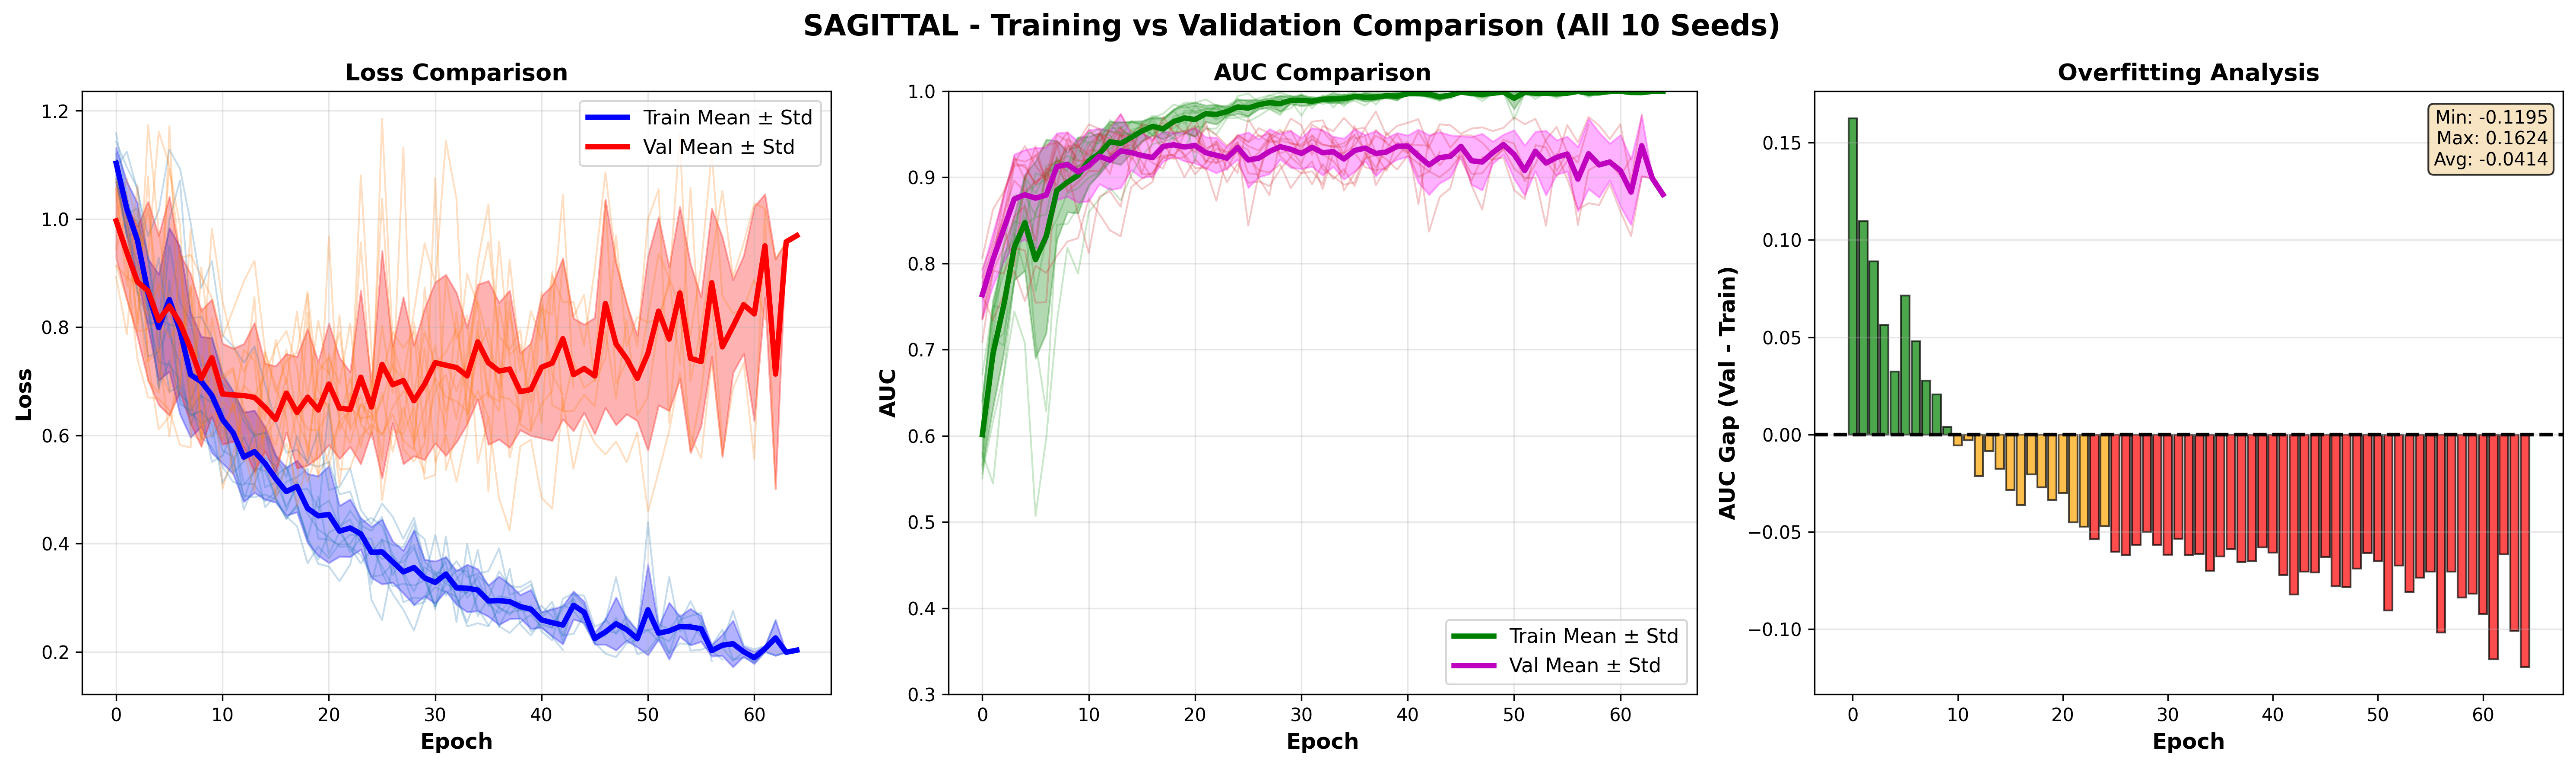
\includegraphics[width=0.88\textwidth]{figs/outputs/VIT_sagittal_entrenamiento_multiseed.png}

\vspace{0.6em}

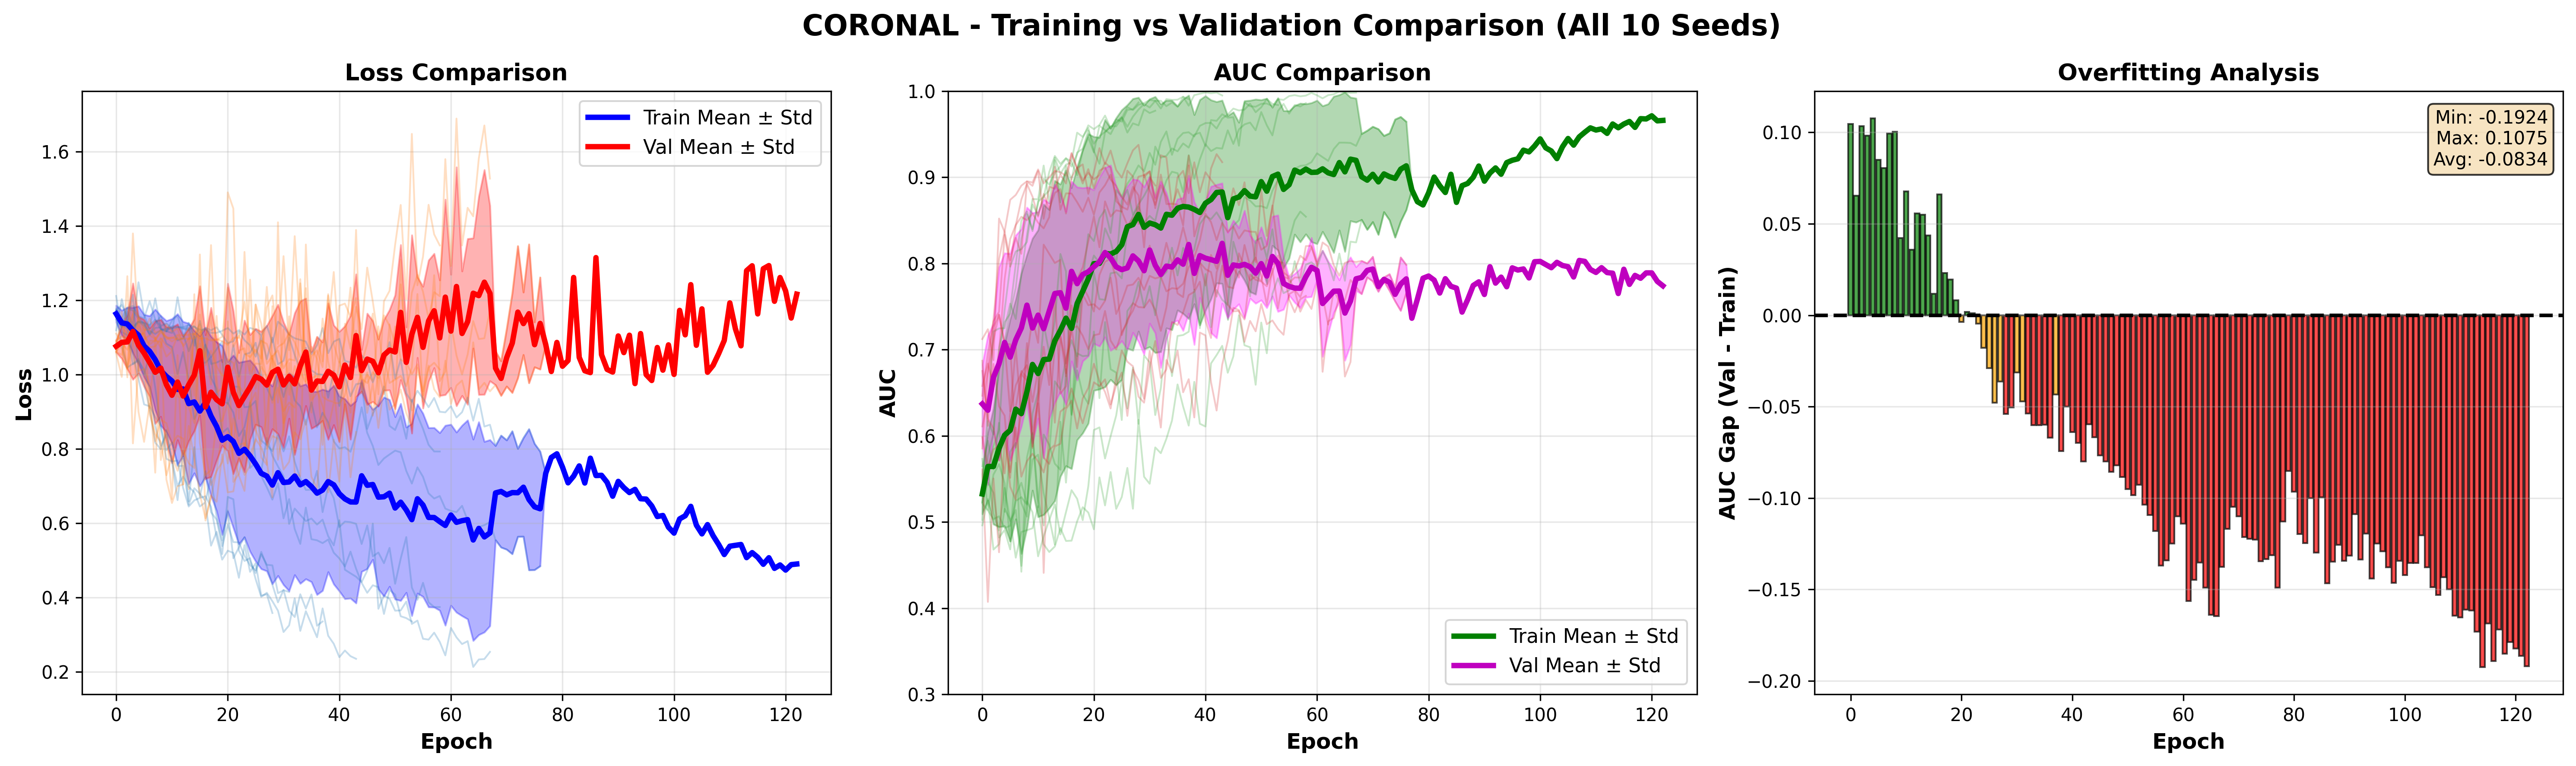
\includegraphics[width=0.88\textwidth]{figs/outputs/VIT_coronal_entrenamiento_multiseed.png}

\vspace{0.6em}

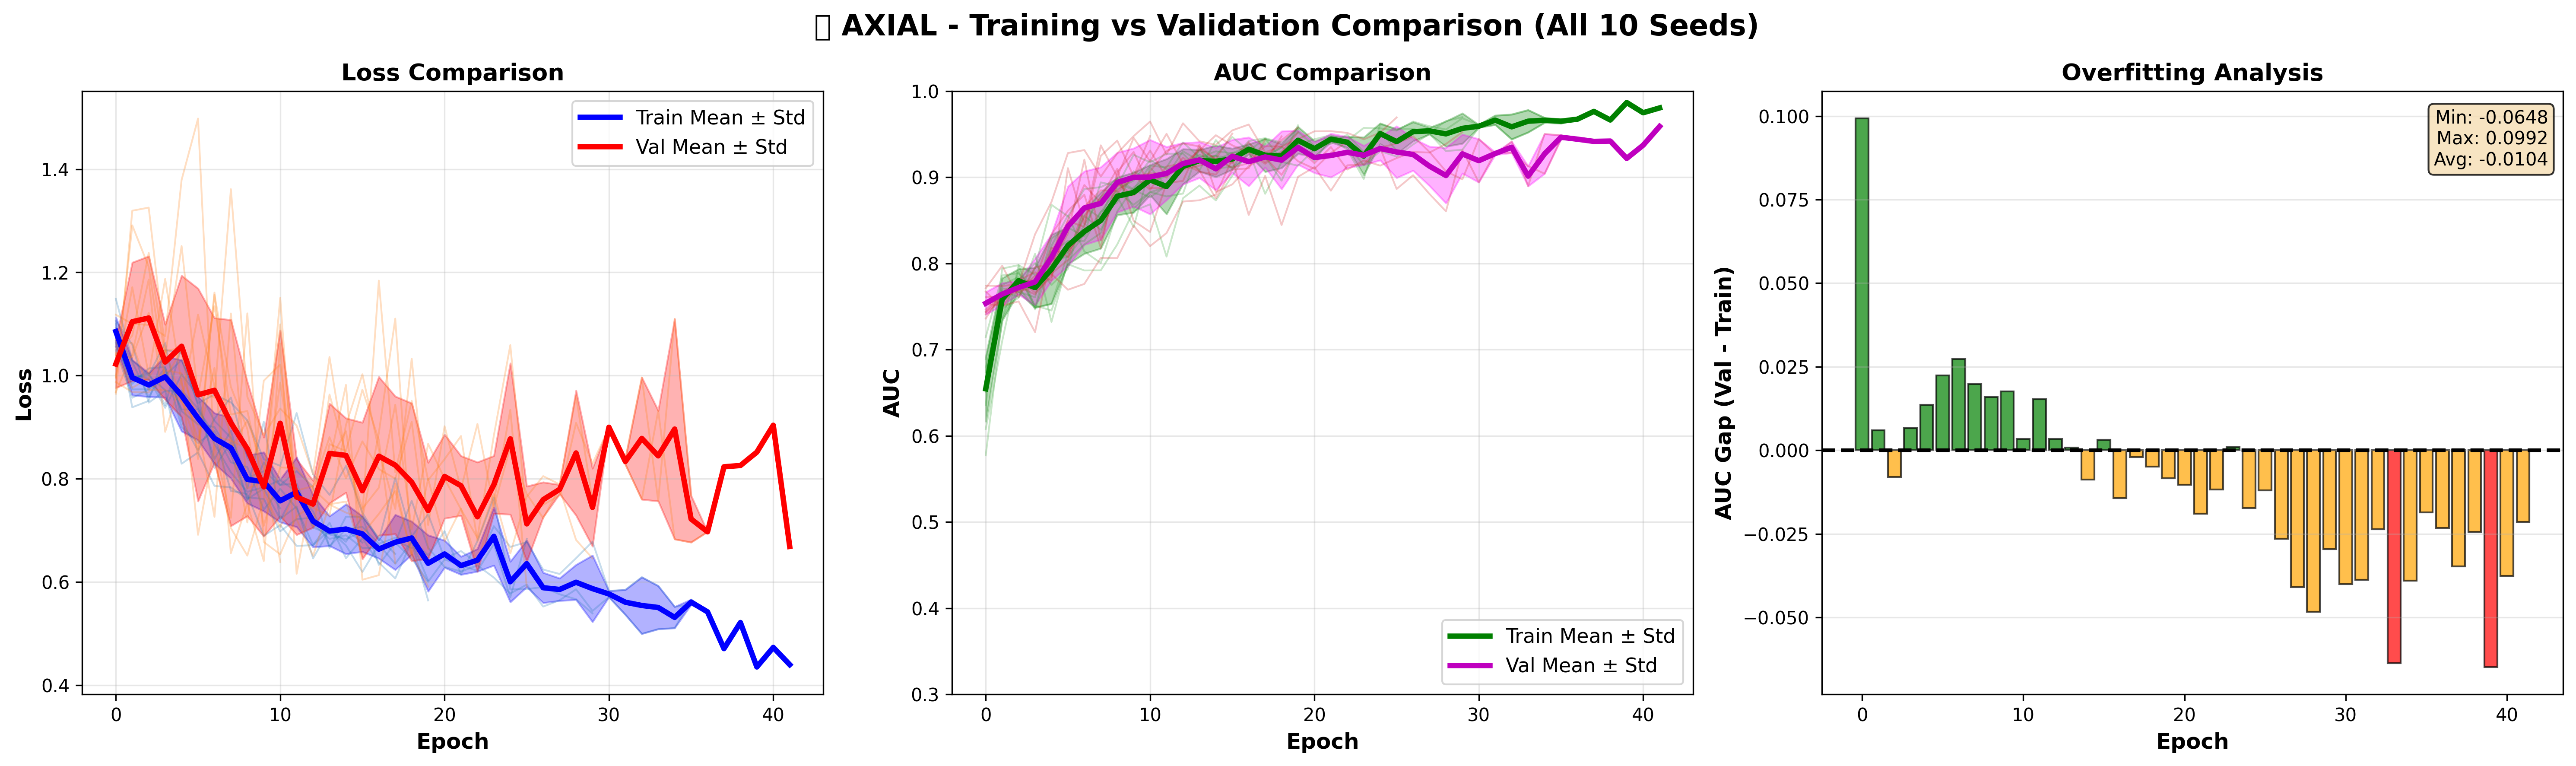
\includegraphics[width=0.88\textwidth]{figs/outputs/VIT_axial_entrenamiento_multiseed.png}
\caption{Evolución del entrenamiento multi-semilla de ViT-Small en los planos sagital, coronal y axial. Cada figura recoge, de izquierda a derecha, la pérdida de entrenamiento y de validación, el AUC de entrenamiento y de validación, y el análisis de sobreajuste ---la brecha de AUC entre validación y entrenamiento (Val $-$ Train) en cada época---; las curvas representan la media $\pm$ desviación típica de las diez semillas.}
\label{fig:vit_multiseed_training}
\end{figure}

En los planos sagital y axial las curvas de validación son suaves y reproducibles entre semillas, con una brecha respecto a la pérdida de entrenamiento que crece de forma controlada, signo de un sobreajuste moderado bien gestionado por el \textit{early stopping}. En el plano coronal, en cambio, las trayectorias de validación se solapan de forma mucho más dispersa entre semillas y presentan oscilaciones más marcadas, lo que es coherente con la elevada desviación estándar observada en el boxplot y con la mayor dificultad de localizar el LCA en esta proyección.

% (fusionado en Rendimiento por vista)

Tras el análisis multi-semilla, se fijó un modelo por plano utilizando únicamente la información de validación. Posteriormente, el conjunto de test se utilizó solo para estimar el rendimiento final. Los resultados se muestran en la Tabla~\ref{tab:vit_individual}.

\begin{table}[H]
\centering
\small
\caption{Rendimiento de los modelos ViT-Small fijados por plano anatómico utilizando únicamente validación.}
\label{tab:vit_individual}
\begin{tabularx}{\textwidth}{
>{\raggedright\arraybackslash}X
>{\centering\arraybackslash}m{2.2cm}
>{\centering\arraybackslash}m{2.2cm}
}
\toprule
\textbf{Plano anatómico} &
\textbf{AUC validación} &
\textbf{AUC test} \\
\midrule
Sagital & 0.9764 & 0.8932 \\
Coronal & 0.9377 & 0.8882 \\
Axial   & 0.9695 & 0.9380 \\
\bottomrule
\end{tabularx}
\end{table}

Los modelos fijados de ViT-Small alcanzaron un rendimiento competitivo en los tres planos. En validación destacaron los planos sagital y axial, mientras que las métricas de test se reportan exclusivamente como evaluación final.

\subsection{Ensamble multi-vista calibrado}

El ensamble ViT-Small utilizó un umbral de $\tau = 0.3804$, seleccionado en validación. La Tabla~\ref{tab:ensemble_vitbase_metricas} resume las métricas principales.

\begin{table}[H]
\centering
\scriptsize
\caption{Rendimiento del ensamble multi-vista basado en ViT-Small con umbral calibrado en validación (resultados en validación y test).}
\label{tab:ensemble_vitbase_metricas}
\begin{tabularx}{\textwidth}{
>{\raggedright\arraybackslash}X
>{\centering\arraybackslash}m{1.15cm}
>{\centering\arraybackslash}m{1.15cm}
>{\centering\arraybackslash}m{1.15cm}
>{\centering\arraybackslash}m{1.15cm}
>{\centering\arraybackslash}m{1.15cm}
>{\centering\arraybackslash}m{1.15cm}
>{\centering\arraybackslash}m{1.15cm}
}
\toprule
\textbf{Conjunto} &
\textbf{AUC} &
\textbf{Acc} &
\textbf{Prec.} &
\textbf{Recall} &
\textbf{Esp.} &
\textbf{F1} &
\textbf{Umbral} \\
\midrule
Validación & 0.9837 & 0.9362 & 0.7500 & 1.0000 & 0.9211 & 0.8571 & 0.3804 \\
Test       & 0.9433 & 0.8663 & 0.6552 & 0.8837 & 0.8611 & 0.7525 & 0.3804 \\
\bottomrule
\end{tabularx}
\end{table}


\begin{figure}[H]
\centering
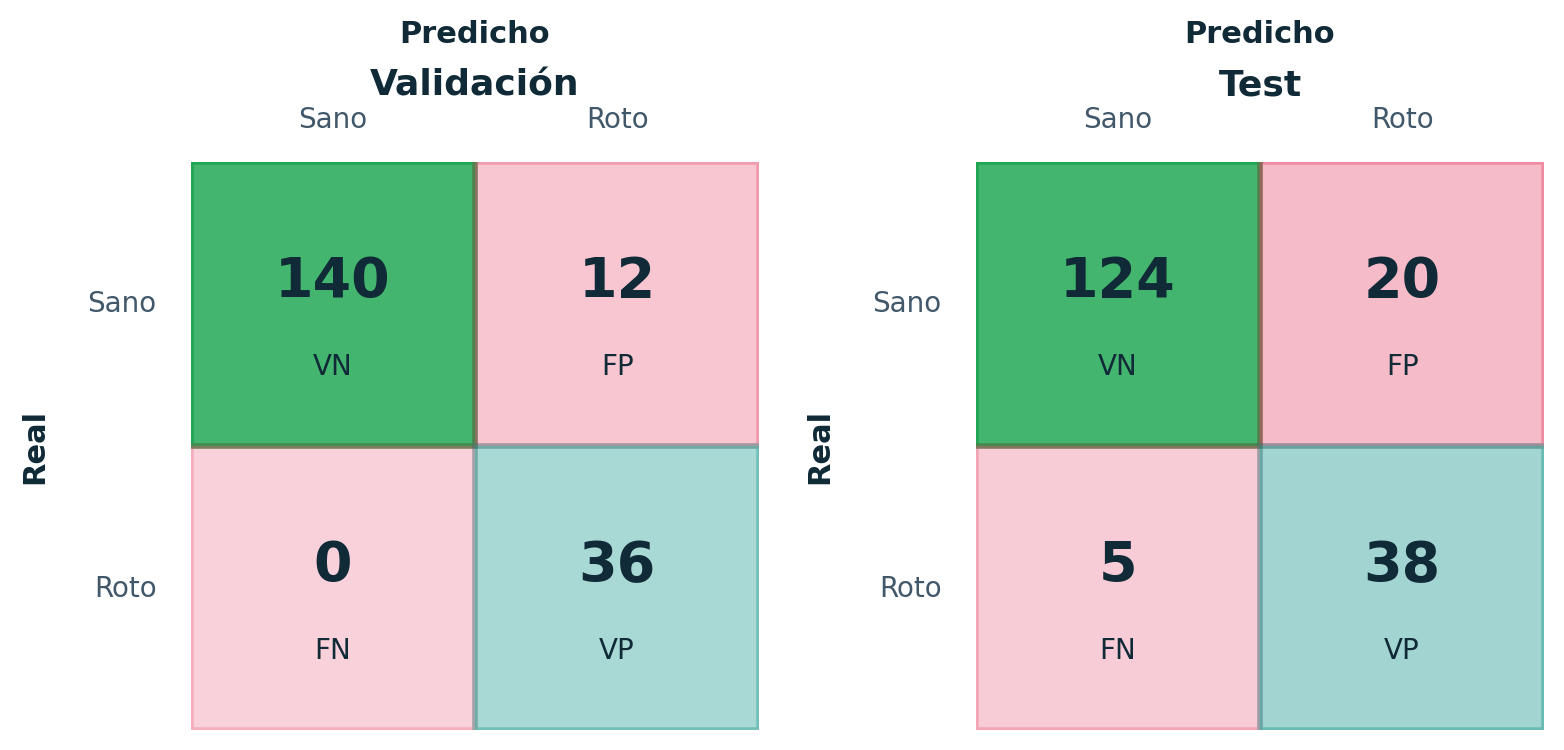
\includegraphics[width=0.92\textwidth]{figs/outputs/VIT_cm_grafica.png}
\caption{Matrices de confusión del ensamble ViT-Small en validación (izquierda) y test (derecha), con el umbral clínico fijado en validación.}
\label{fig:ensemble_vitbase_confusion}
\end{figure}

En validación, el ensamble ViT-Small detectó las 36 roturas presentes sin ningún falso negativo (sensibilidad de 1.0). En la evaluación final sobre test alcanzó un AUC de 0.9433 con 5 falsos negativos, mostrando un buen equilibrio entre sensibilidad y discriminación global.

La Figura~\ref{fig:vit_best_training} resume las curvas de mejores checkpoints de ViT-Small.

\begin{figure}[H]
\centering
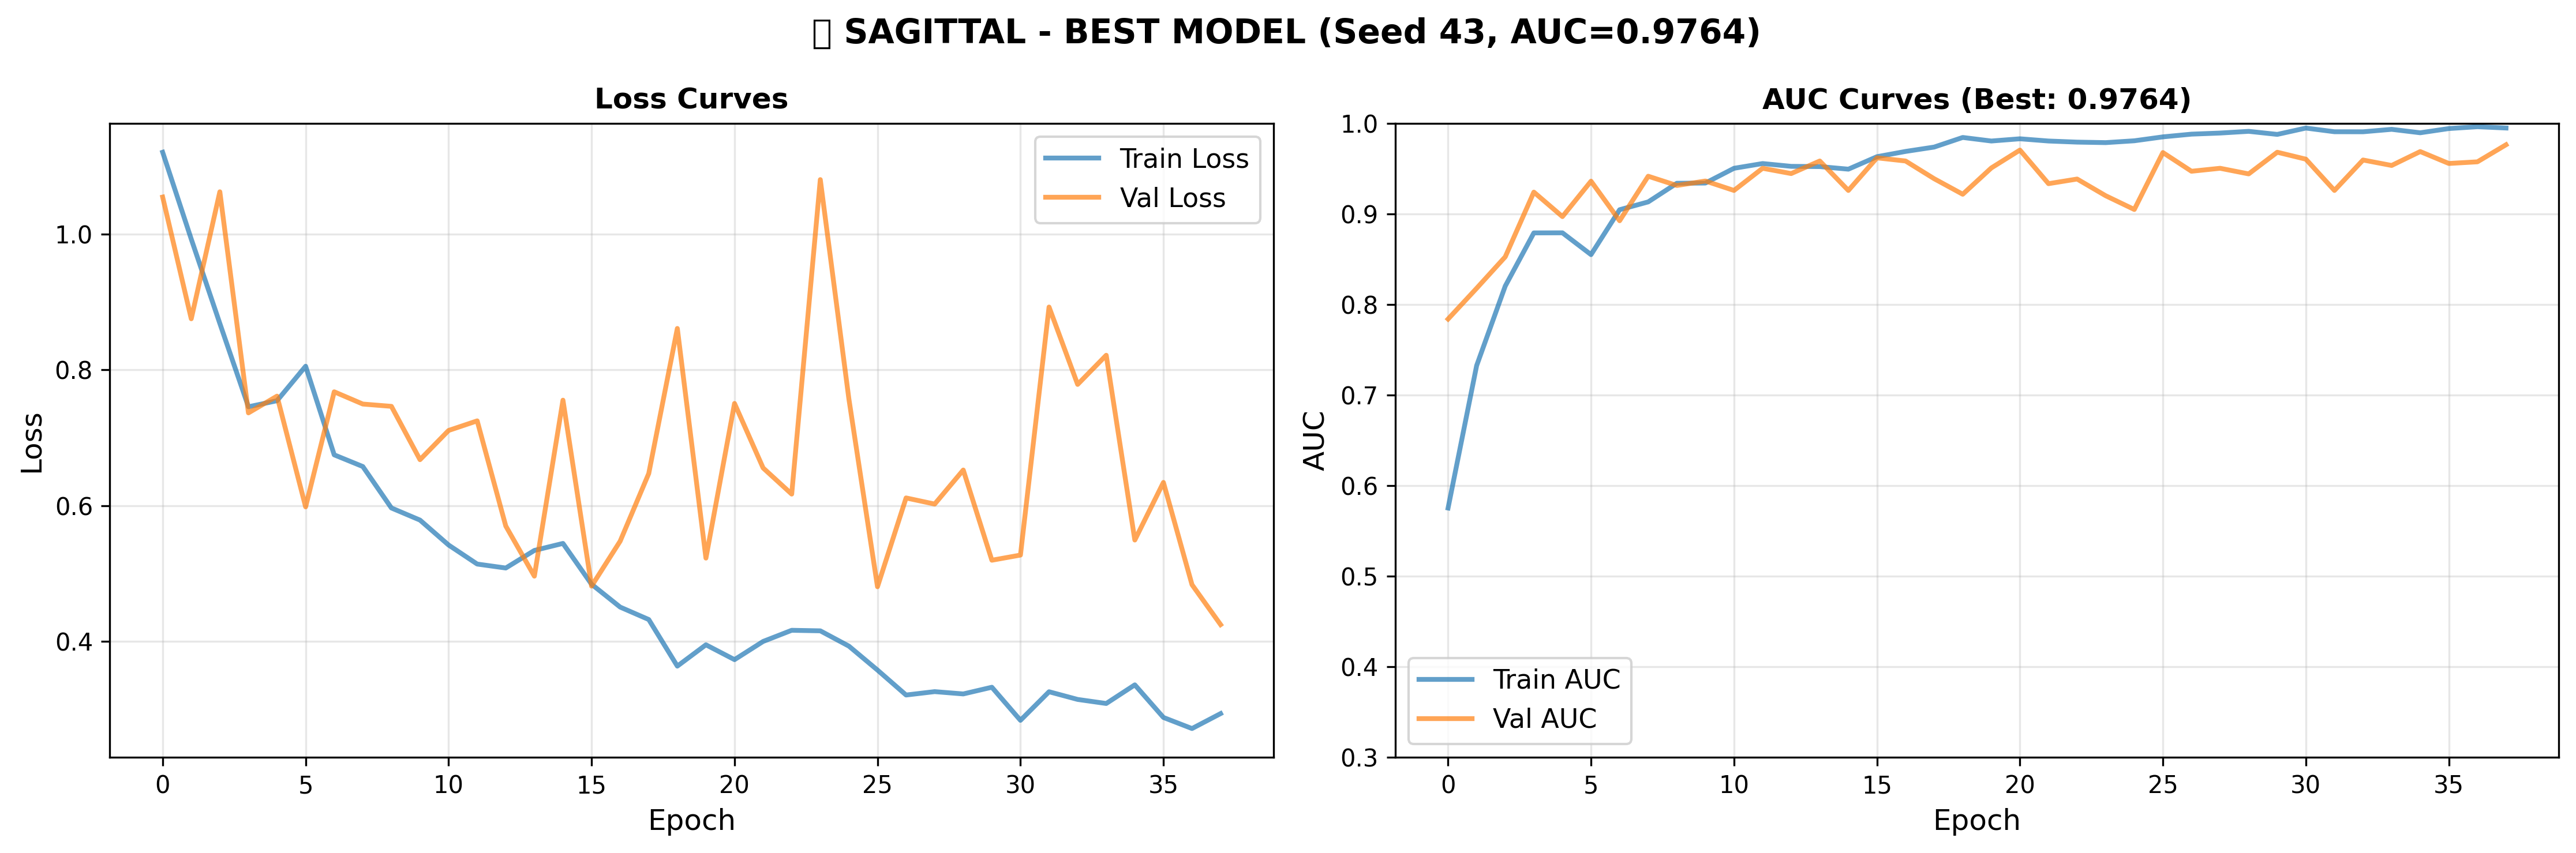
\includegraphics[width=0.88\textwidth]{figs/outputs/VIT_sagittal_best.png}

\vspace{0.6em}

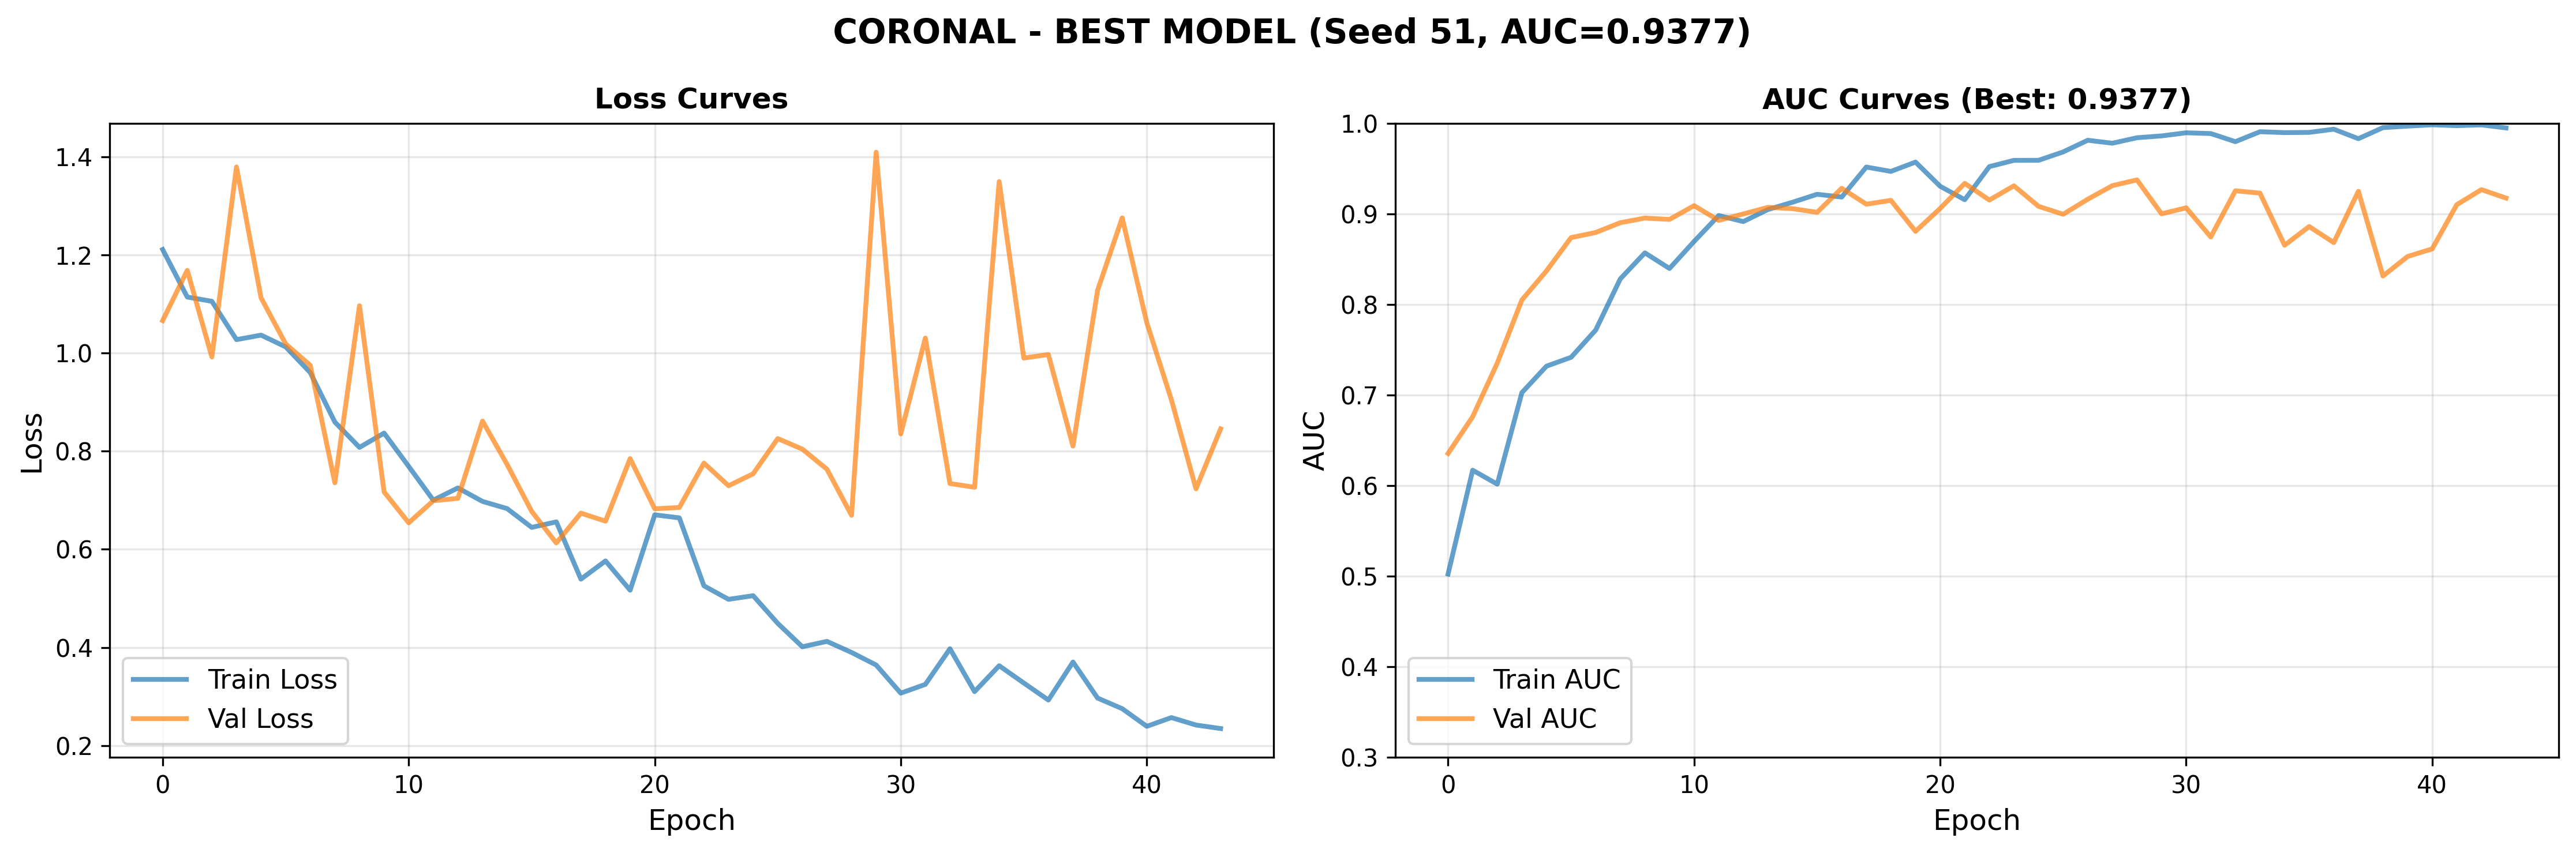
\includegraphics[width=0.88\textwidth]{figs/outputs/VIT_coronal_best.png}

\vspace{0.6em}

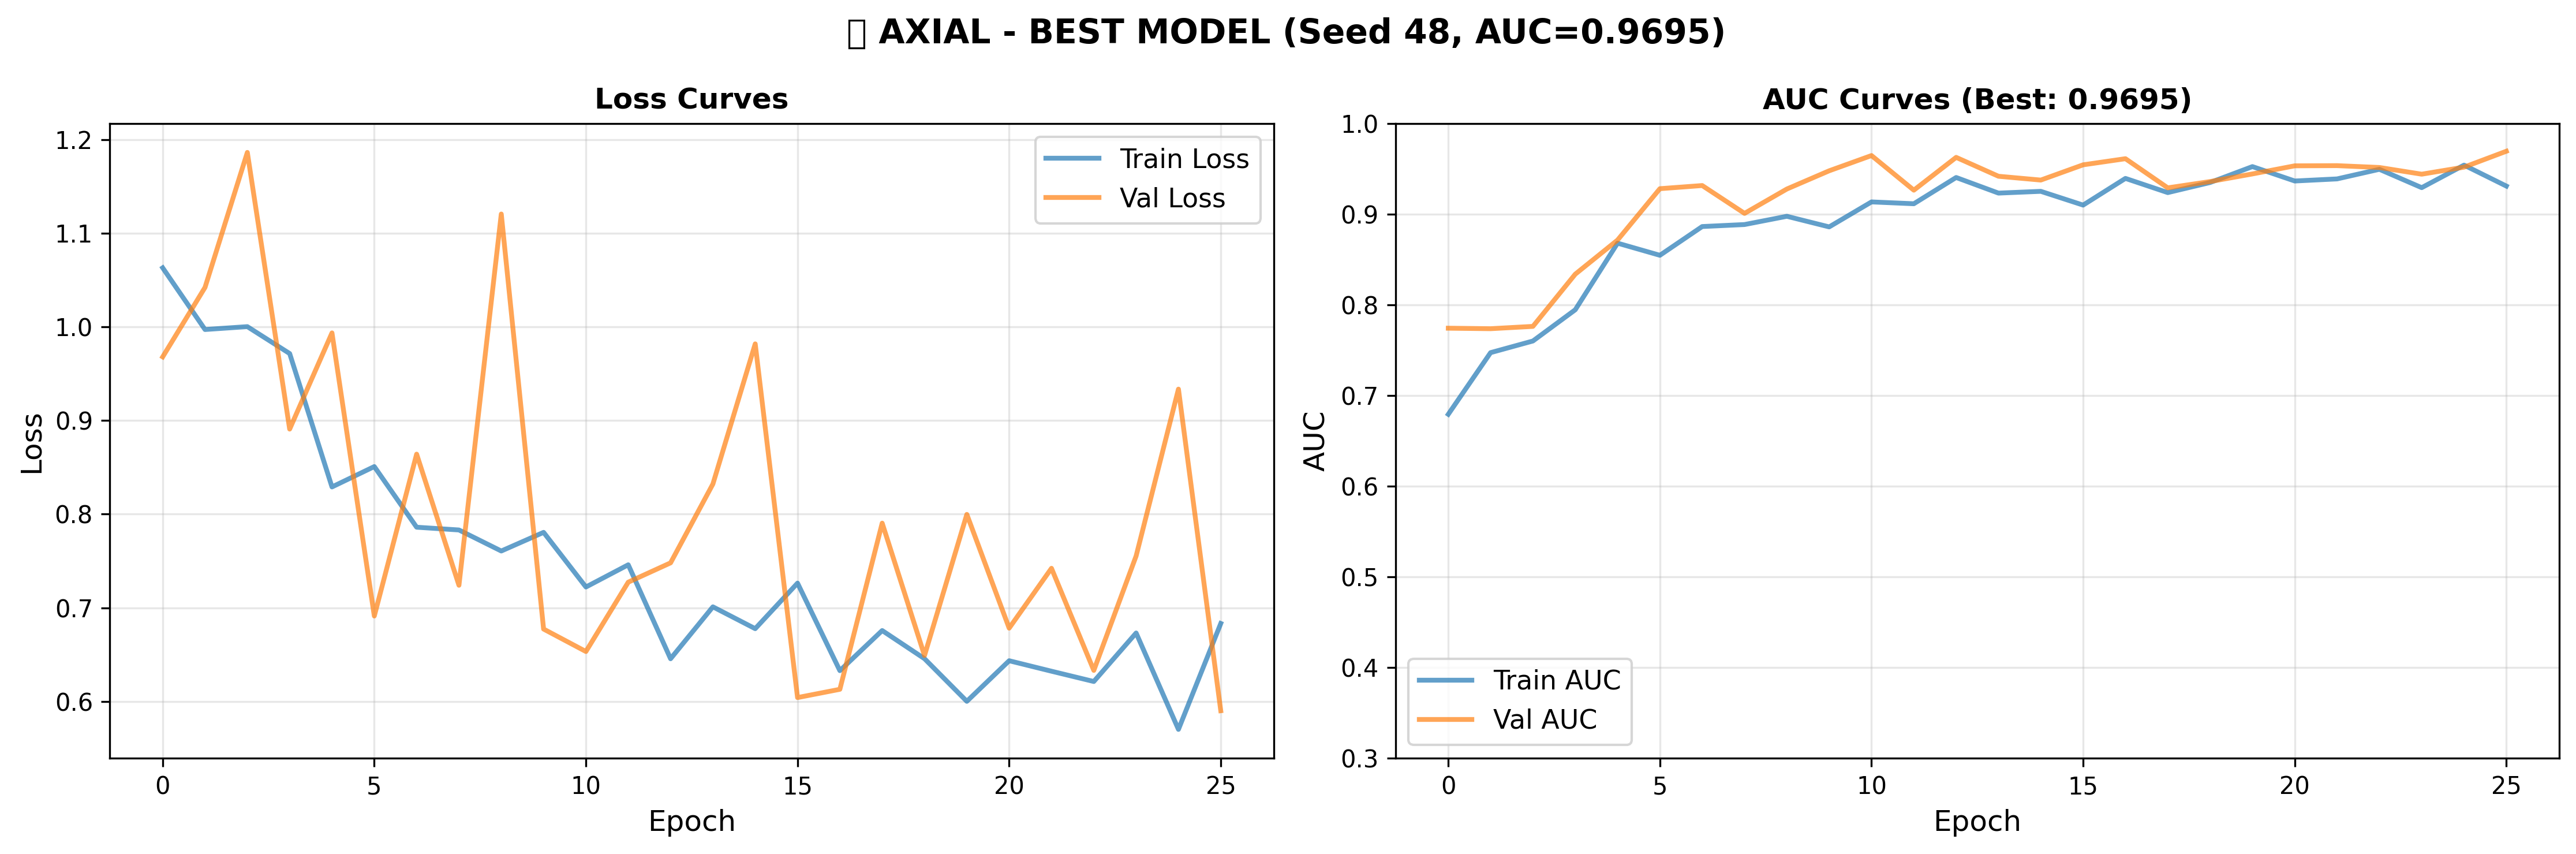
\includegraphics[width=0.88\textwidth]{figs/outputs/VIT_axial_best.png}
\caption{Curvas de entrenamiento de los mejores checkpoints de ViT-Small por plano anatómico.}
\label{fig:vit_best_training}
\end{figure}

% -------------------------------------------------------------------------
% RESULTADOS SWIN-SMALL
% -------------------------------------------------------------------------

\section{Swin-Tiny}
\label{subsec:resultados_swin_small}

\textit{Swin Transformer Tiny} combina atención local mediante ventanas desplazadas con una representación jerárquica.

\subsection{Rendimiento por vista: estabilidad multi-semilla y checkpoint fijado}

Al igual que en ResNet50 y ViT-Small, Swin-Tiny fue evaluado mediante diez semillas independientes por plano anatómico. La Figura~\ref{fig:multiseed_swin_small} resume la distribución del AUC de validación por plano.

\begin{figure}[H]
\centering
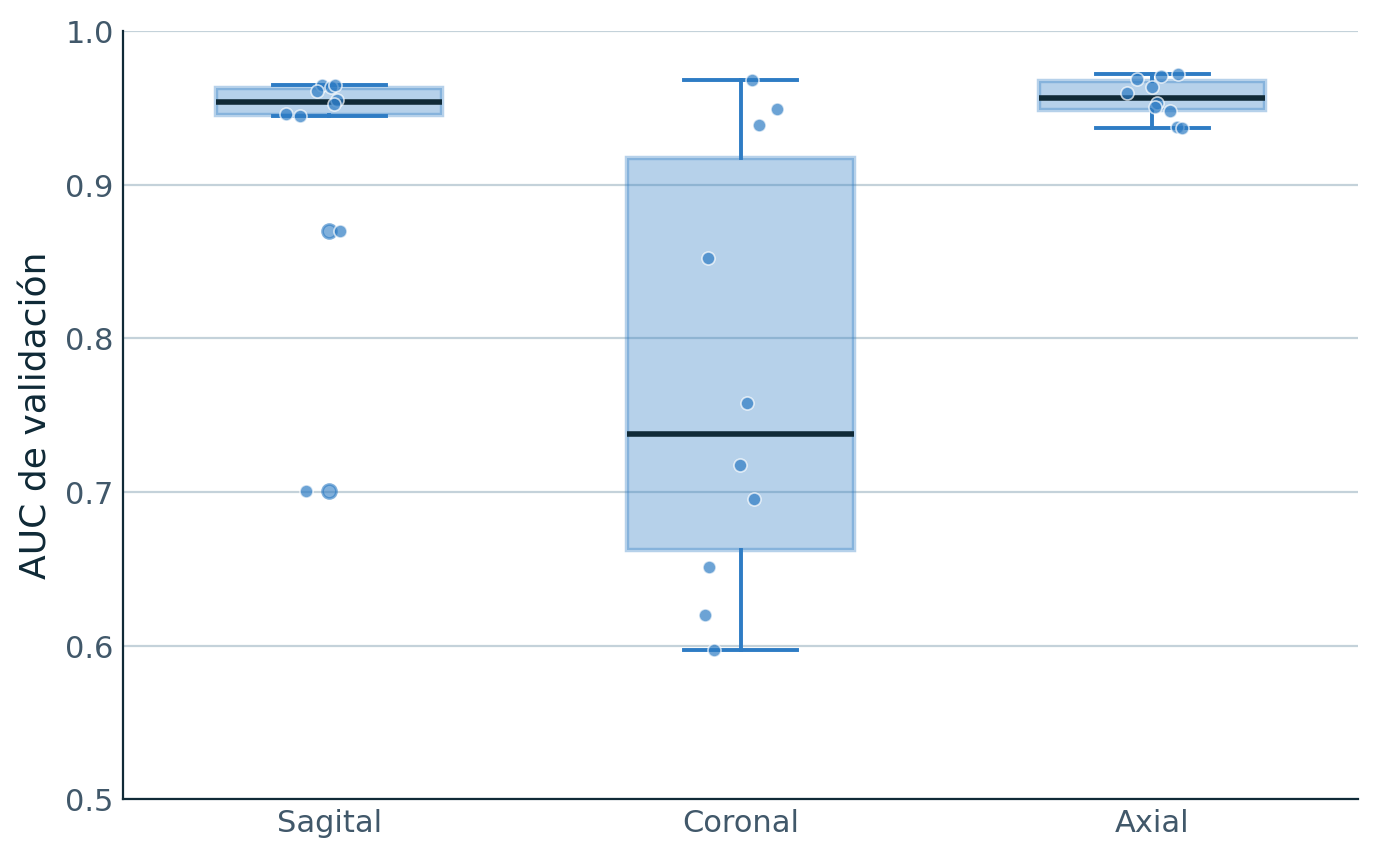
\includegraphics[width=0.82\textwidth]{figs/outputs/SWIN_boxplot.png}
\caption{Distribución del AUC de \textbf{validación} de Swin-Tiny sobre las diez semillas (42--51) en cada plano anatómico. Cada punto corresponde a una semilla; la caja representa el rango intercuartílico y la línea central, la mediana. La amplitud de la caja del plano coronal evidencia la inestabilidad de esta proyección.}
\label{fig:multiseed_swin_small}
\end{figure}

El plano axial fue el más estable, con un AUC medio de 0.9560 y una desviación estándar de 0.0123. En cambio, el plano coronal mostró la mayor variabilidad, con una desviación estándar de 0.1348 y un AUC mínimo de 0.5970, prácticamente equivalente al azar. Esto indica que, mientras algunas semillas alcanzaron un rendimiento elevado (AUC máximo de 0.9684), otras no llegaron a converger: el modelo colapsó hacia una solución trivial, próxima a predecir siempre la clase mayoritaria.

Este comportamiento puede explicarse por la conjunción de varios factores. Por una parte, el plano coronal es el más difícil para localizar el LCA de forma consistente, ya que el ligamento aparece a menudo parcialmente representado y con mayor interferencia de los tejidos circundantes; además, en este plano se procesan $K=10$ cortes, frente a los $5$ del sagital, lo que aumenta la proporción de información poco discriminativa. Por otra parte, la atención local por ventanas de Swin-Tiny depende de que la señal relevante esté espacialmente bien localizada; cuando la inicialización no consigue fijar esa señal débil en las primeras épocas, el entrenamiento queda atrapado en la solución trivial y no escapa de ella, de ahí los casos con AUC cercano a 0.5. Esta fragilidad refuerza la necesidad del análisis multi-semilla y justifica el papel del ensamble multi-vista, en el que la aportación más débil del plano coronal se compensa con la de los planos sagital y axial.

Por todo ello, la interpretación de Swin-Tiny debe basarse en el conjunto de evidencias: estabilidad en validación, comportamiento del ensamble y evaluación externa.

La Figura~\ref{fig:swin_multiseed_training} muestra la evolución del entrenamiento multi-semilla de Swin-Tiny en los tres planos anatómicos.

\begin{figure}[H]
\centering
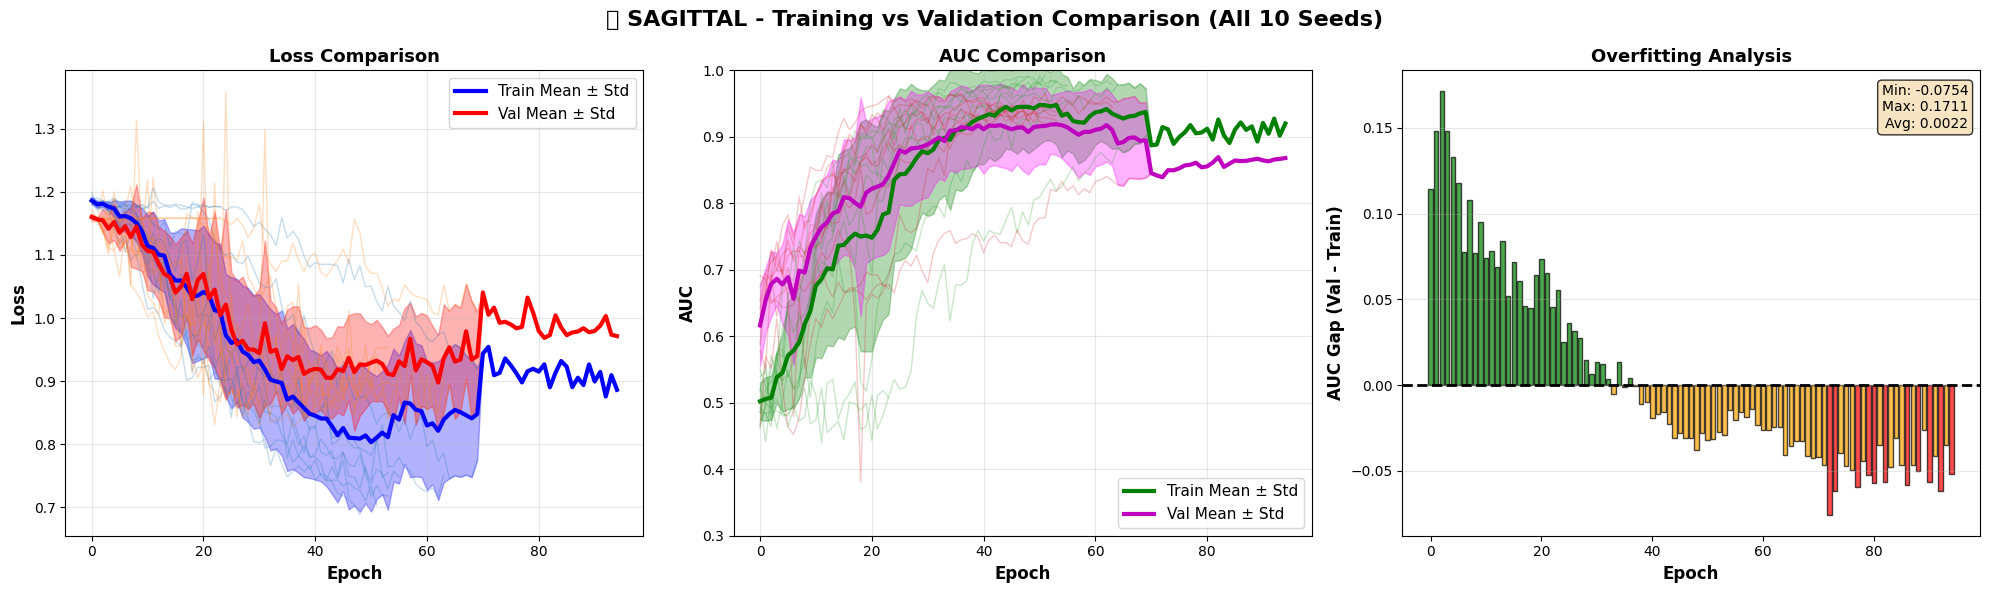
\includegraphics[width=0.88\textwidth]{figs/outputs/SWIN_sagittal_entrenamiento_multiseed.png}

\vspace{0.6em}

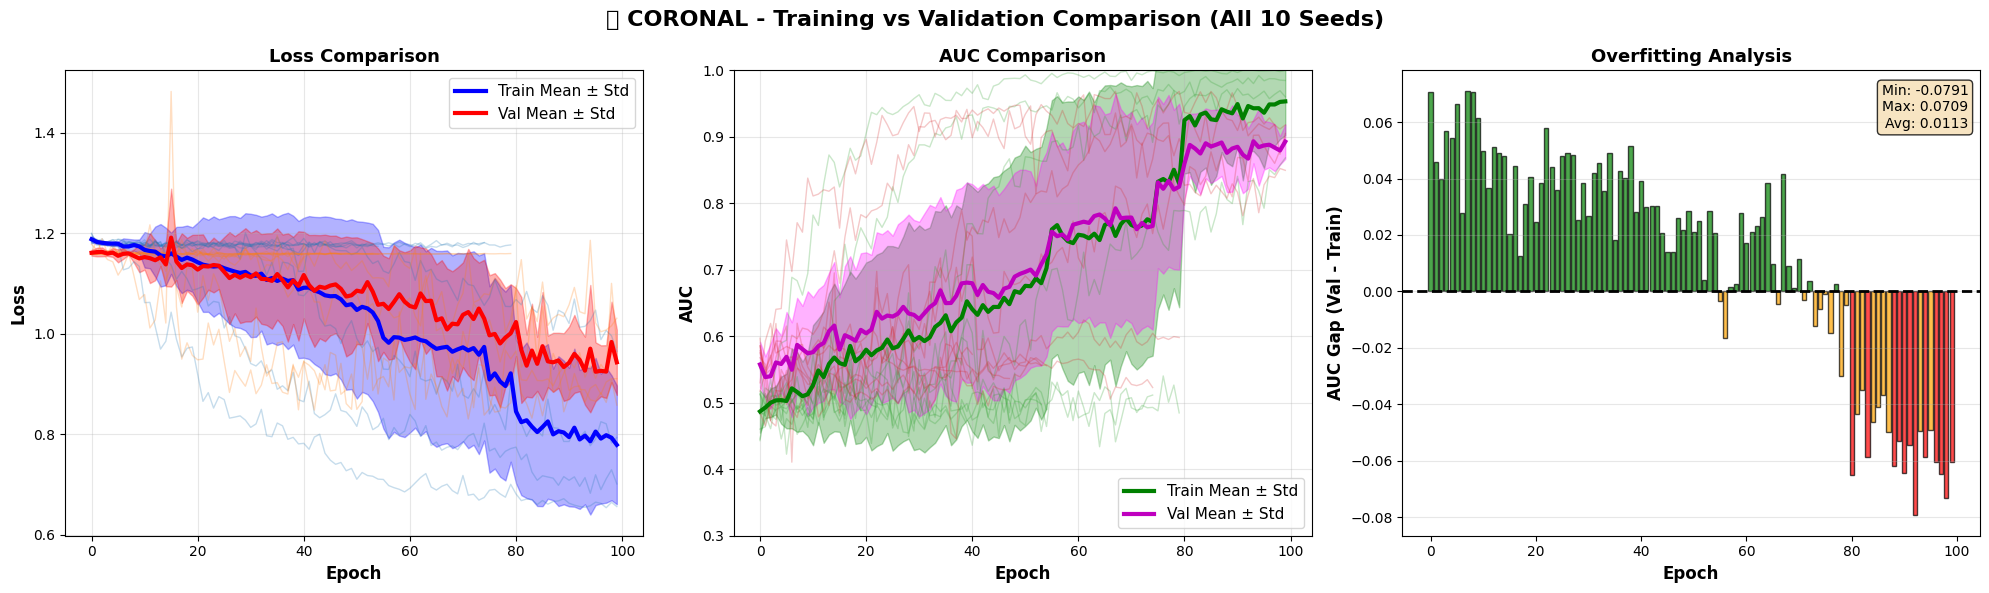
\includegraphics[width=0.88\textwidth]{figs/outputs/SWIN_coronal_entrenamiento_multiseed.png}

\vspace{0.6em}

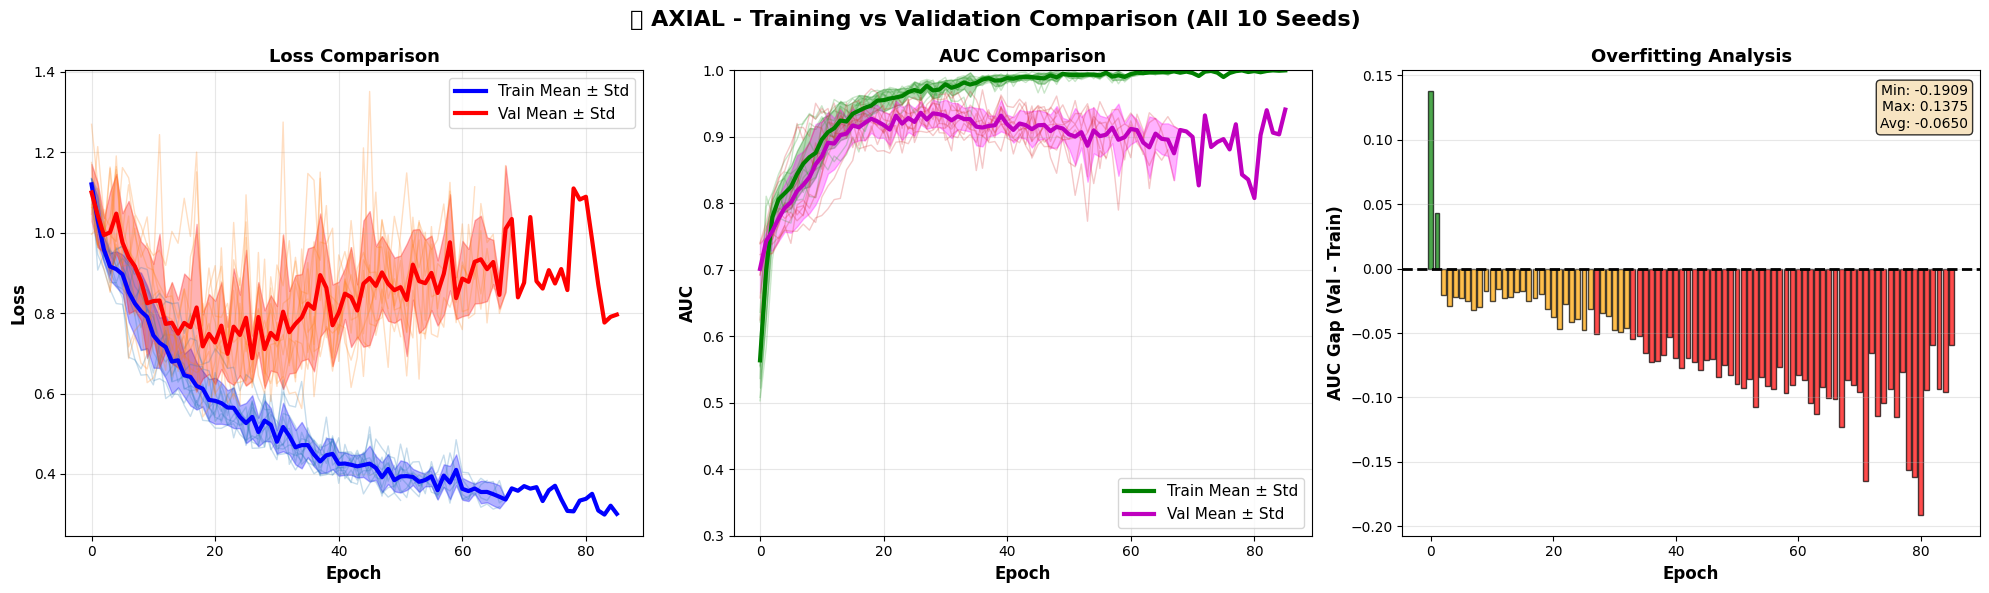
\includegraphics[width=0.88\textwidth]{figs/outputs/SWIN_axial_entrenamiento_multiseed.png}
\caption{Evolución del entrenamiento multi-semilla de Swin-Tiny en los planos sagital, coronal y axial. Cada figura recoge, de izquierda a derecha, la pérdida de entrenamiento y de validación, el AUC de entrenamiento y de validación, y el análisis de sobreajuste ---la brecha de AUC entre validación y entrenamiento (Val $-$ Train) en cada época---; las curvas representan la media $\pm$ desviación típica de las diez semillas.}
\label{fig:swin_multiseed_training}
\end{figure}

Estas curvas hacen visible el fenómeno descrito: en el plano axial las trayectorias de validación de las distintas semillas se agrupan de forma compacta y descienden de manera estable, mientras que en el coronal aparecen semillas cuya pérdida de validación apenas mejora respecto al inicio ---el modelo queda atrapado en la solución trivial--- junto a otras que sí convergen. Donde la convergencia es correcta, la brecha entre entrenamiento y validación crece de forma contenida y el \textit{early stopping} fija el checkpoint antes de que el sobreajuste se acentúe; los casos no convergentes, en cambio, se descartan de forma natural al seleccionar por AUC de validación.

% (fusionado en Rendimiento por vista)

A partir del análisis multi-semilla se fijaron los checkpoints utilizados en cada plano anatómico para construir el ensamble, empleando únicamente información procedente de validación. De este modo, las métricas del ensamble no se presentan como una ejecución aislada, sino como el resultado de combinar modelos definidos antes de consultar el conjunto de test.

La Figura~\ref{fig:swin_best_training} recoge las curvas de entrenamiento de los checkpoints seleccionados para Swin-Tiny.

\begin{figure}[H]
\centering
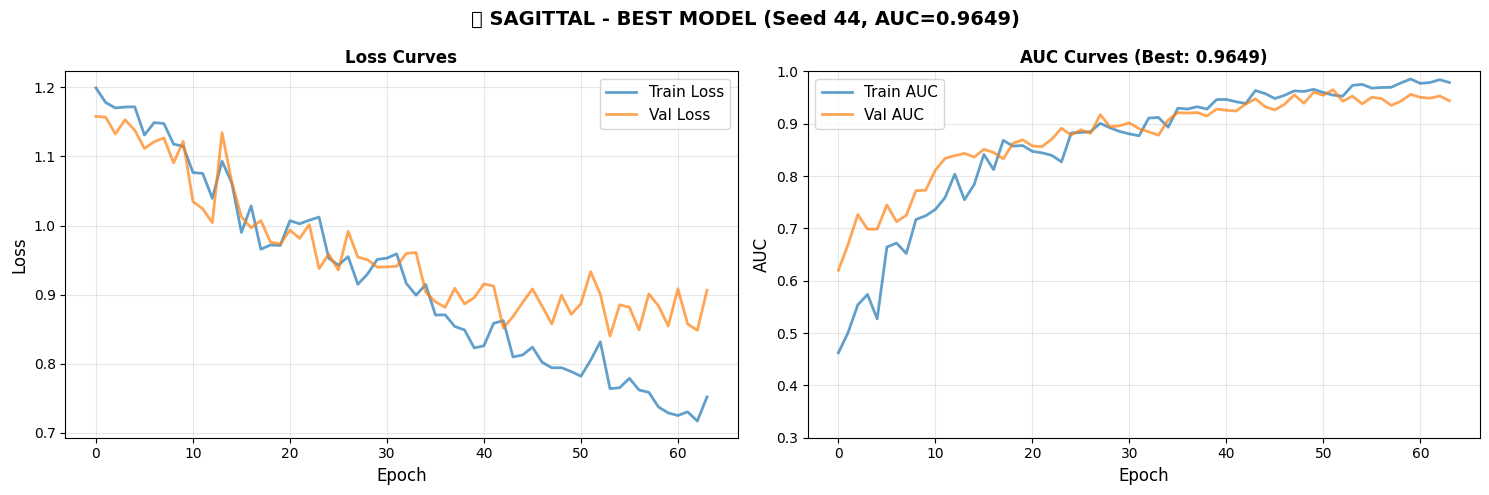
\includegraphics[width=0.88\textwidth]{figs/outputs/SWIN_sagittal_best.png}

\vspace{0.6em}

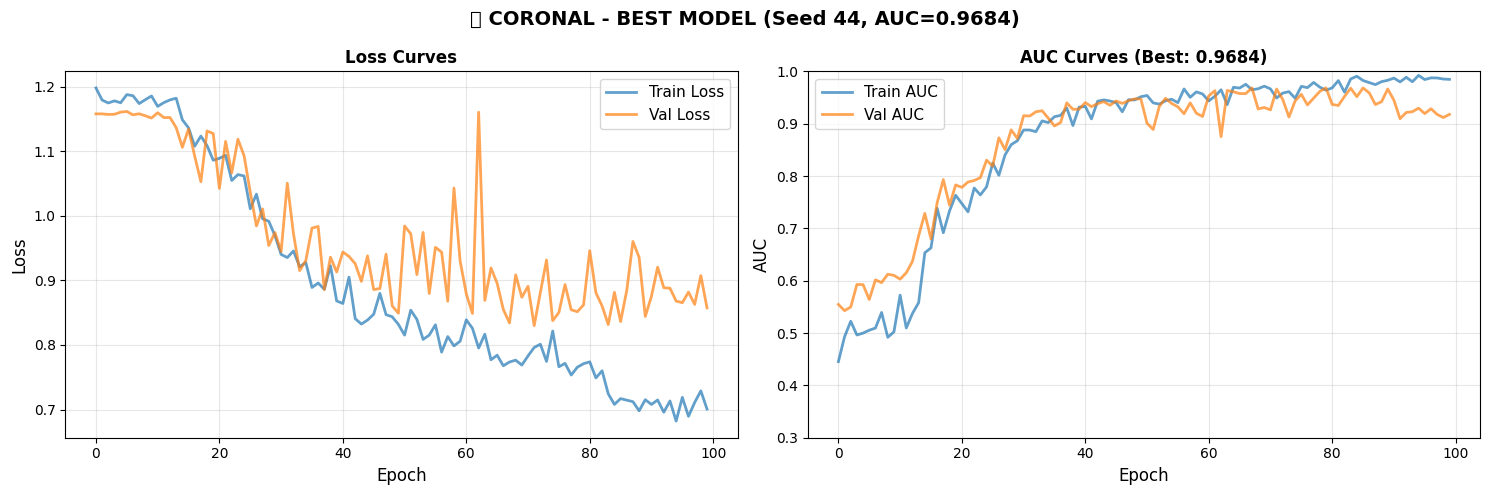
\includegraphics[width=0.88\textwidth]{figs/outputs/SWIN_coronal_best.png}

\vspace{0.6em}

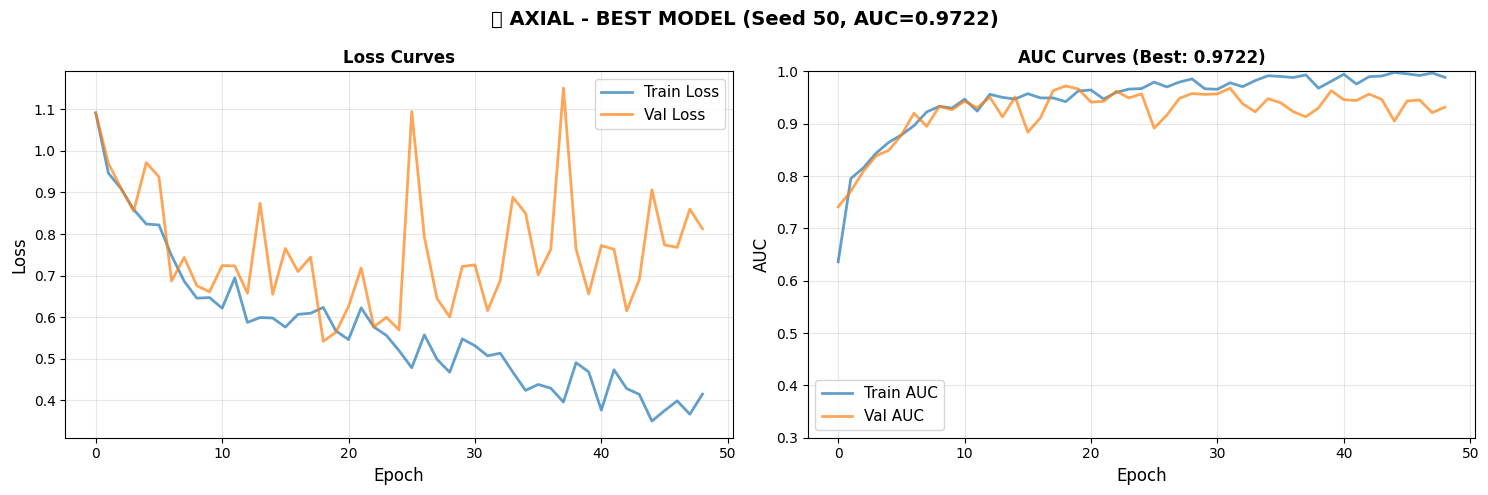
\includegraphics[width=0.88\textwidth]{figs/outputs/SWIN_axial_best.png}
\caption{Curvas de entrenamiento de los mejores checkpoints de Swin-Tiny por plano anatómico.}
\label{fig:swin_best_training}
\end{figure}

\subsection{Ensamble multi-vista calibrado}

El ensamble Swin-Tiny se construyó mediante promedio simple de las probabilidades de los tres planos. El umbral seleccionado en validación fue $\tau = 0.3734$. Las métricas se presentan en la Tabla~\ref{tab:ensemble_swin_metricas}.

\begin{table}[H]
\centering
\scriptsize
\caption{Rendimiento del ensamble multi-vista basado en Swin-Tiny con umbral calibrado en validación (resultados en validación y test).}
\label{tab:ensemble_swin_metricas}
\begin{tabularx}{\textwidth}{
>{\raggedright\arraybackslash}X
>{\centering\arraybackslash}m{1.15cm}
>{\centering\arraybackslash}m{1.15cm}
>{\centering\arraybackslash}m{1.15cm}
>{\centering\arraybackslash}m{1.15cm}
>{\centering\arraybackslash}m{1.15cm}
>{\centering\arraybackslash}m{1.15cm}
>{\centering\arraybackslash}m{1.15cm}
}
\toprule
\textbf{Conjunto} &
\textbf{AUC} &
\textbf{Acc} &
\textbf{Prec.} &
\textbf{Recall} &
\textbf{Esp.} &
\textbf{F1} &
\textbf{Umbral} \\
\midrule
Validación & 0.9837 & 0.9362 & 0.7609 & 0.9722 & 0.9276 & 0.8537 & 0.3734 \\
Test       & 0.9536 & 0.8556 & 0.6290 & 0.9070 & 0.8403 & 0.7429 & 0.3734 \\
\bottomrule
\end{tabularx}
\end{table}


\begin{figure}[H]
\centering
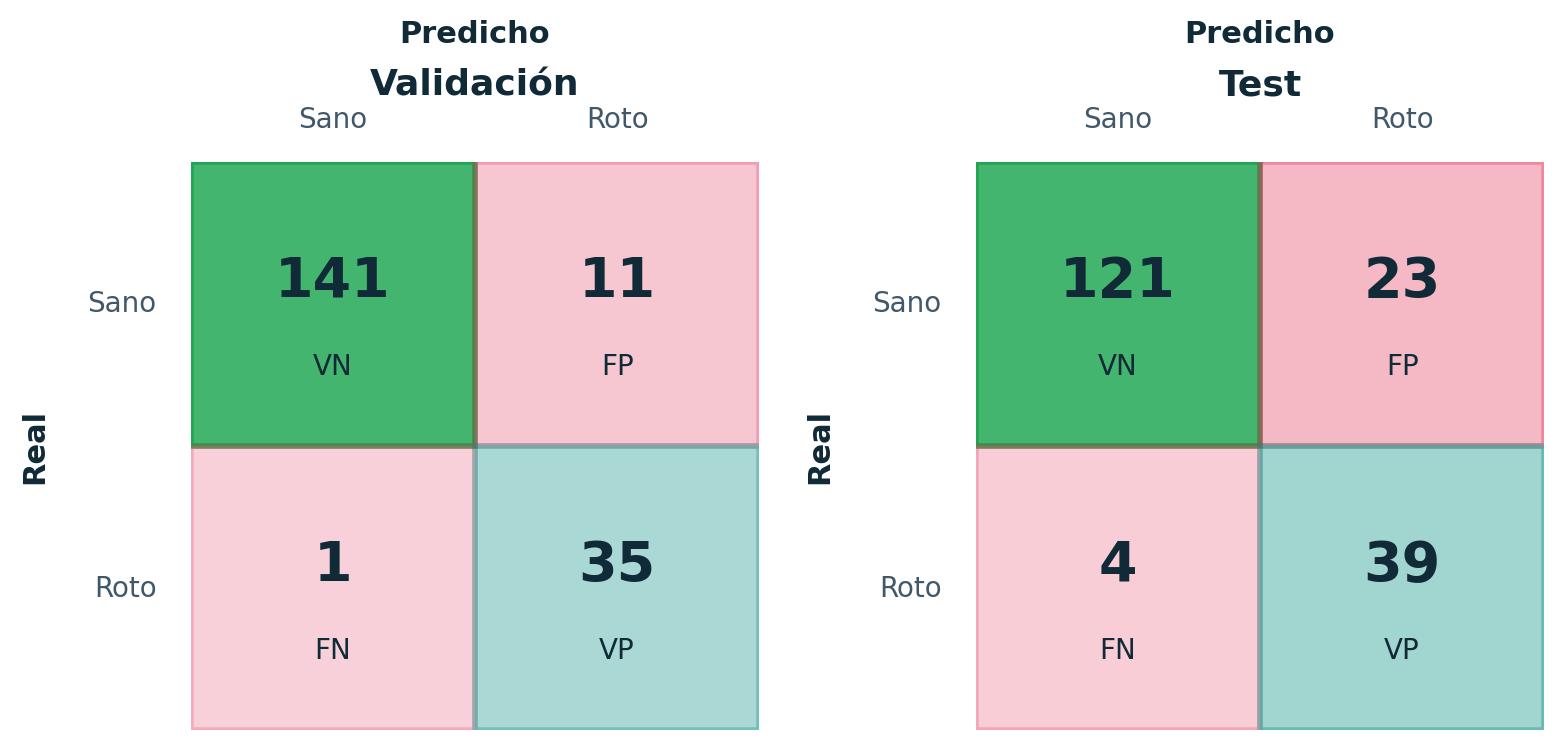
\includegraphics[width=0.92\textwidth]{figs/outputs/SWIN_cm_grafica.png}
\caption{Matrices de confusión del ensamble Swin-Tiny en validación (izquierda) y test (derecha), con el umbral clínico fijado en validación.}
\label{fig:ensemble_swin_confusion}
\end{figure}

En la evaluación final sobre test, Swin-Tiny obtuvo una sensibilidad de 0.9070, detectando 39 de las 43 roturas presentes y dejando 4 falsos negativos. El coste de este punto operativo fue un aumento de los falsos positivos, con 23 controles clasificados como positivos, lo que redujo su precisión y especificidad respecto a ViT-Small.

Desde una perspectiva clínica, este comportamiento puede ser favorable cuando se prioriza la reducción de falsos negativos. Sin embargo, no debe interpretarse como una mejora universal en todas las métricas ni como una elección definitiva basada en test.

% -------------------------------------------------------------------------
% COMPARATIVA FINAL EN MRNET
% -------------------------------------------------------------------------

\section{Comparativa y análisis}
\label{sec:comparativa_analisis}
\label{subsec:comparativa_final_mrnet}

La comparación entre ensambles debe interpretarse separando dos niveles. En primer lugar, la Tabla~\ref{tab:comparativa_ensembles_mrnet_val} resume el rendimiento en validación, que es el conjunto utilizado para fijar los umbrales y describir el comportamiento operativo esperado. En segundo lugar, la Tabla~\ref{tab:comparativa_ensembles_mrnet_test} muestra la evaluación final sobre el conjunto de test de MRNet, utilizado únicamente para estimar la capacidad de generalización bajo las decisiones previamente fijadas.

Esta comparación permite distinguir entre rendimiento discriminativo global, medido mediante AUC, y rendimiento clínico bajo el umbral seleccionado, medido mediante sensibilidad, especificidad, precisión y F1-score.

\begin{table}[H]
\centering
\scriptsize
\caption{Comparativa de los ensambles multi-vista en el conjunto de validación de MRNet.}
\label{tab:comparativa_ensembles_mrnet_val}
\begin{tabularx}{\textwidth}{
>{\raggedright\arraybackslash}X
>{\centering\arraybackslash}m{1.05cm}
>{\centering\arraybackslash}m{1.05cm}
>{\centering\arraybackslash}m{1.05cm}
>{\centering\arraybackslash}m{1.05cm}
>{\centering\arraybackslash}m{1.05cm}
>{\centering\arraybackslash}m{1.05cm}
>{\centering\arraybackslash}m{1.05cm}
>{\centering\arraybackslash}m{1.05cm}
}
\toprule
\textbf{Modelo} &
\textbf{AUC} &
\textbf{Acc} &
\textbf{Prec.} &
\textbf{Recall} &
\textbf{Esp.} &
\textbf{F1} &
\textbf{FN} &
\textbf{FP} \\
\midrule
ViT-Small &
\textbf{0.9837} &
\textbf{0.9362} &
0.7500 &
\textbf{1.0000} &
0.9211 &
\textbf{0.8571} &
\textbf{0} &
12 \\

ResNet50 &
0.9836 &
\textbf{0.9362} &
\textbf{0.7609} &
0.9722 &
\textbf{0.9276} &
0.8537 &
1 &
\textbf{11} \\

Swin-Tiny &
\textbf{0.9837} &
\textbf{0.9362} &
\textbf{0.7609} &
0.9722 &
\textbf{0.9276} &
0.8537 &
1 &
\textbf{11} \\
\bottomrule
\end{tabularx}
\end{table}

\begin{table}[H]
\centering
\scriptsize
\caption{Comparativa de los ensambles multi-vista en el conjunto de test de MRNet.}
\label{tab:comparativa_ensembles_mrnet_test}
\begin{tabularx}{\textwidth}{
>{\raggedright\arraybackslash}X
>{\centering\arraybackslash}m{1.05cm}
>{\centering\arraybackslash}m{1.05cm}
>{\centering\arraybackslash}m{1.05cm}
>{\centering\arraybackslash}m{1.05cm}
>{\centering\arraybackslash}m{1.05cm}
>{\centering\arraybackslash}m{1.05cm}
>{\centering\arraybackslash}m{1.05cm}
>{\centering\arraybackslash}m{1.05cm}
}
\toprule
\textbf{Modelo} &
\textbf{AUC} &
\textbf{Acc} &
\textbf{Prec.} &
\textbf{Recall} &
\textbf{Esp.} &
\textbf{F1} &
\textbf{FN} &
\textbf{FP} \\
\midrule
ViT-Small &
0.9433 &
\textbf{0.8663} &
\textbf{0.6552} &
0.8837 &
\textbf{0.8611} &
\textbf{0.7525} &
5 &
\textbf{20} \\

ResNet50 &
\textbf{0.9545} &
0.8556 &
0.6333 &
0.8837 &
0.8472 &
0.7379 &
5 &
22 \\

Swin-Tiny &
0.9536 &
0.8556 &
0.6290 &
\textbf{0.9070} &
0.8403 &
0.7429 &
\textbf{4} &
23 \\
\bottomrule
\end{tabularx}
\end{table}

En validación, el ensamble ViT-Small alcanzó una sensibilidad perfecta (detectó las 36 roturas, sin falsos negativos), mientras que ResNet50 y Swin-Tiny obtuvieron un punto operativo con un falso negativo y once falsos positivos. En test, ResNet50 obtuvo el mayor AUC, ViT-Small mostró mayor exactitud, precisión, especificidad y F1-score, y Swin-Tiny alcanzó la mayor sensibilidad.

La Figura~\ref{fig:roc_ensembles_mrnet_val} agrupa las curvas ROC de validación de los tres ensambles, y la Figura~\ref{fig:roc_ensembles_mrnet_test} las correspondientes al conjunto de test, para las tres arquitecturas evaluadas.

\begin{figure}[H]
\centering
\begin{minipage}{0.32\textwidth}\centering
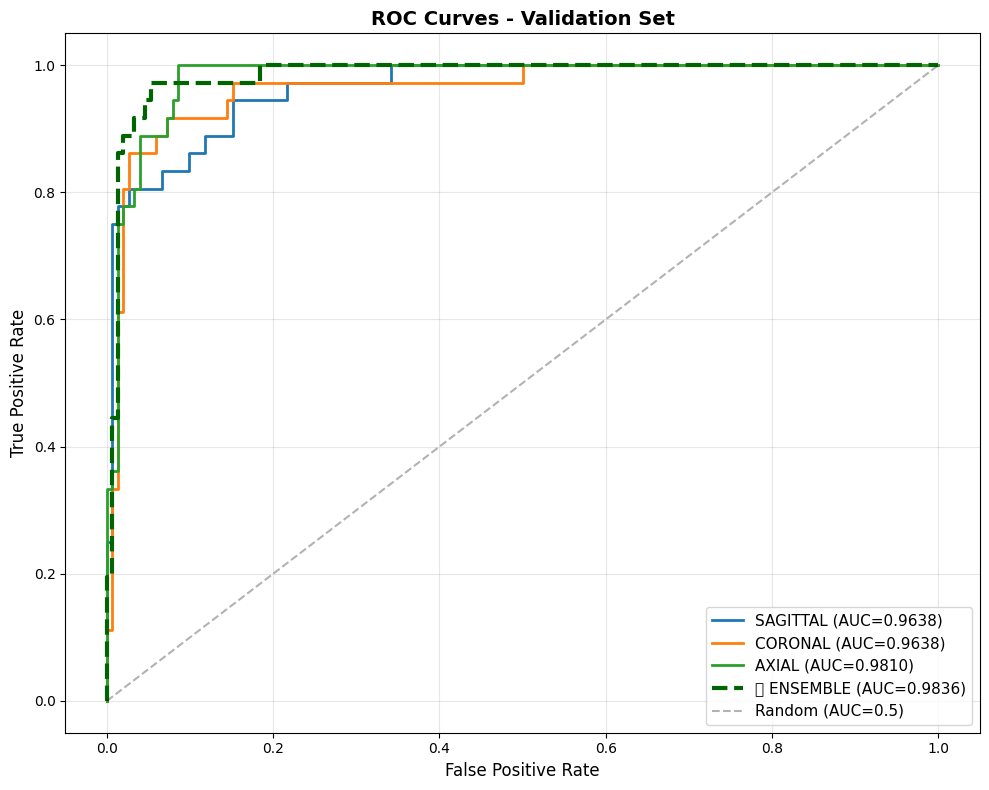
\includegraphics[width=\linewidth]{figs/outputs/CNN_ROC.png}
\end{minipage}\hfill
\begin{minipage}{0.32\textwidth}\centering
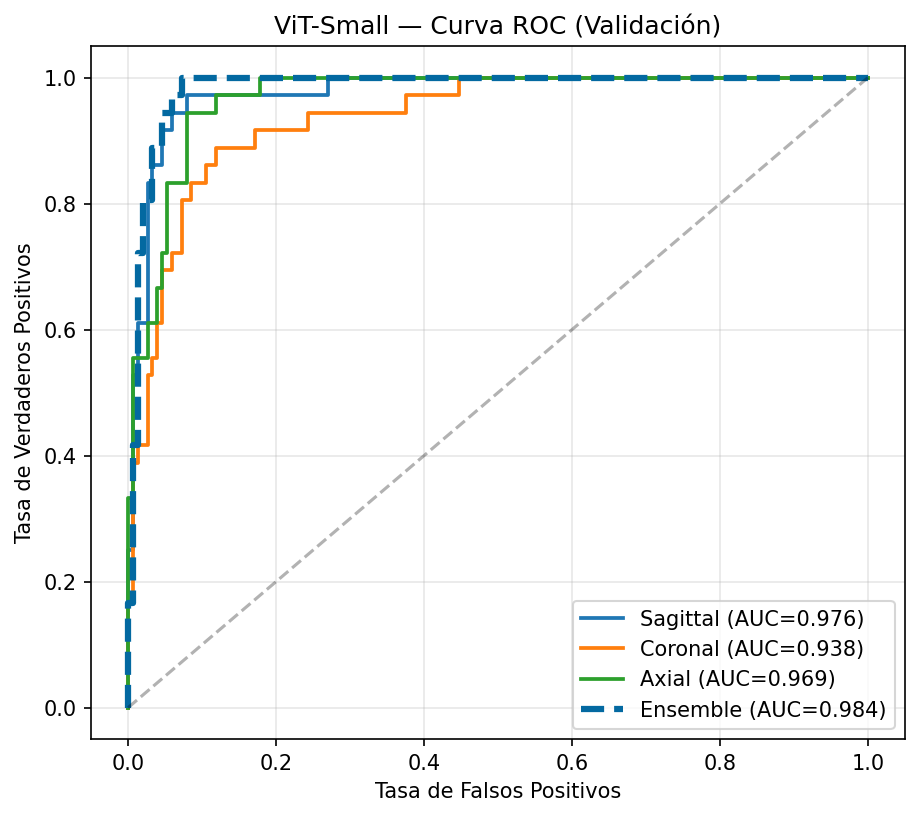
\includegraphics[width=\linewidth]{figs/outputs/VIT_ROC_val.png}
\end{minipage}\hfill
\begin{minipage}{0.32\textwidth}\centering
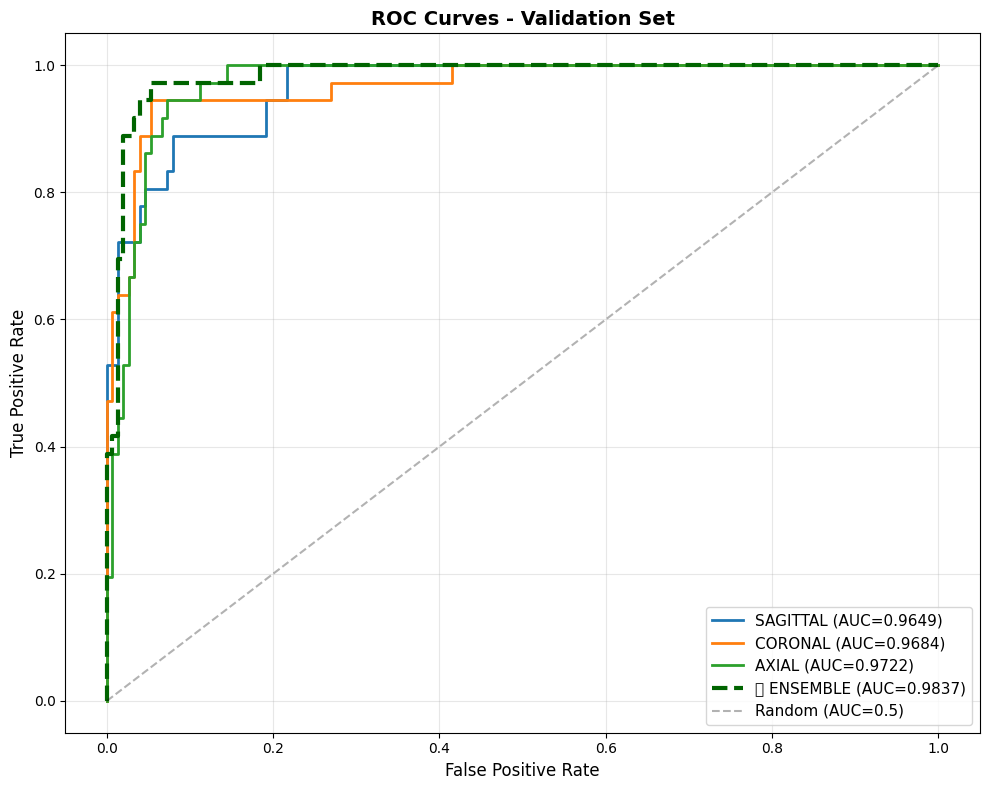
\includegraphics[width=\linewidth]{figs/outputs/SWIN_ROC_val.png}
\end{minipage}
\caption{Curvas ROC de validación de los ensambles ResNet50, ViT-Small y Swin-Tiny en MRNet.}
\label{fig:roc_ensembles_mrnet_val}
\end{figure}

\begin{figure}[H]
\centering
\begin{minipage}{0.32\textwidth}\centering
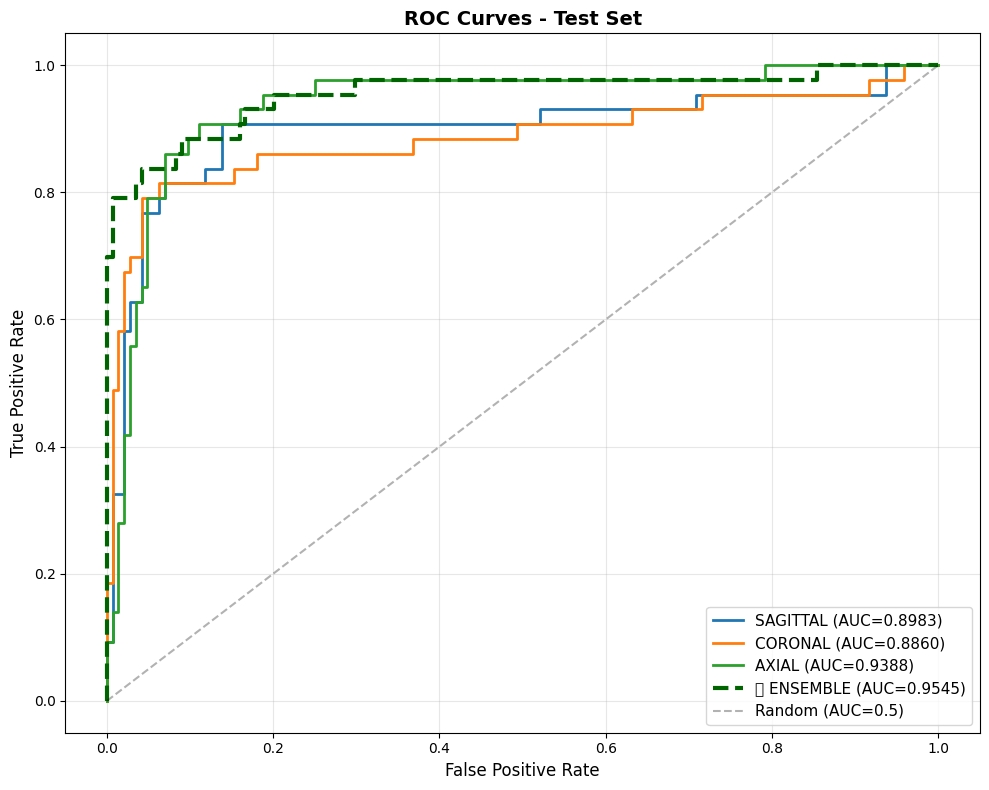
\includegraphics[width=\linewidth]{figs/outputs/CNN_ROC_test.png}
\end{minipage}\hfill
\begin{minipage}{0.32\textwidth}\centering

\includegraphics[width=\linewidth]{figs/outputs/VIT_ROC_test.png}
\end{minipage}\hfill
\begin{minipage}{0.32\textwidth}\centering
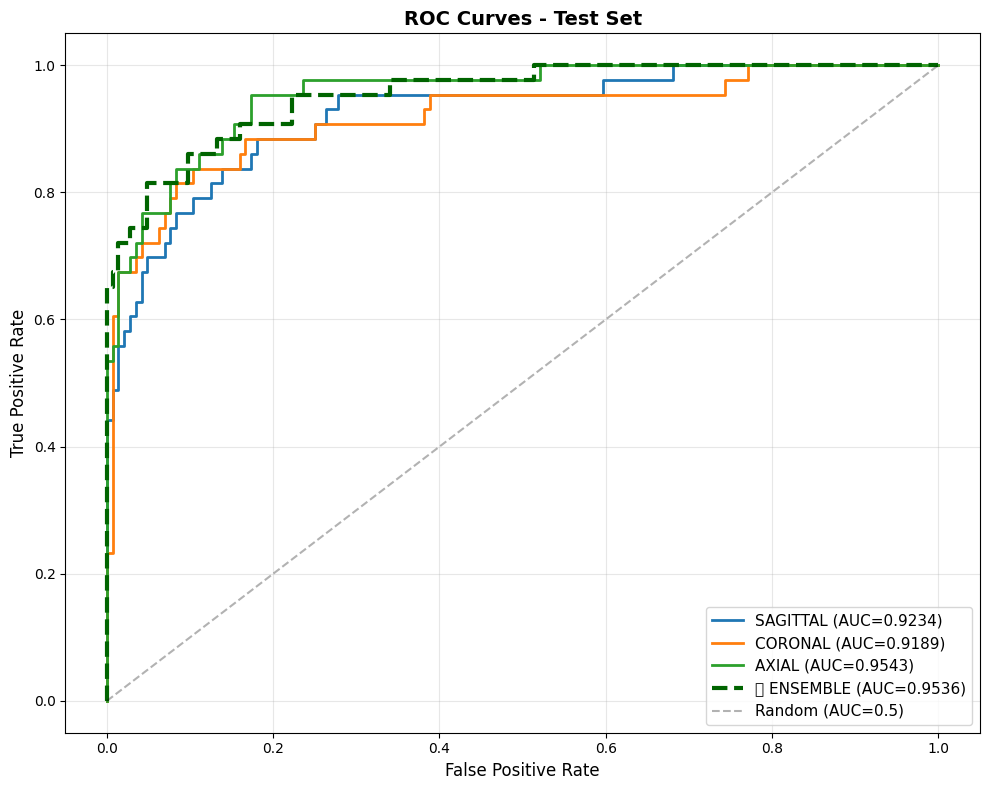
\includegraphics[width=\linewidth]{figs/outputs/SWIN_ROC_test.png}
\end{minipage}
\caption{Curvas ROC de test de los ensambles ResNet50, ViT-Small y Swin-Tiny en MRNet.}
\label{fig:roc_ensembles_mrnet_test}
\end{figure}

En consecuencia, no se propone una selección definitiva de un único modelo a partir del conjunto de test. La comparación en validación permite justificar el comportamiento operativo sin usar test para tomar decisiones, mientras que la comparación en test permite describir compromisos finales entre discriminación global, sensibilidad y falsos positivos.

% -------------------------------------------------------------------------
% FALSOS NEGATIVOS COMUNES
% -------------------------------------------------------------------------

\subsection{Análisis de los falsos negativos comunes}
\label{subsec:falsos_negativos_comunes}

Un falso negativo, es decir, un estudio con rotura real del LCA clasificado como sano, constituye el error más relevante en este dominio clínico, pues implica no detectar una lesión presente. Para comprender la naturaleza de los errores residuales del sistema se analizaron los falsos negativos compartidos por las tres arquitecturas, bajo la hipótesis de que un caso que los tres modelos ---entrenados de forma independiente y con \textit{backbones} de naturaleza muy distinta--- clasifican erróneamente en el mismo sentido difícilmente se explica por una limitación particular de una arquitectura concreta.

Del conjunto de test de MRNet, únicamente tres estudios fueron clasificados como negativos por los tres ensambles de forma simultánea: los casos 0080, 0087 y 0521. La Tabla~\ref{tab:fn_comunes} recoge las probabilidades asignadas por cada arquitectura a estos tres casos.

\begin{table}[H]
\centering
\small
\caption{Probabilidad de rotura asignada por cada ensamble a los tres falsos negativos comunes del conjunto de test. La etiqueta real de los tres casos es rotura del LCA (positivo).}
\label{tab:fn_comunes}
\begin{tabularx}{\textwidth}{
>{\centering\arraybackslash}X
>{\centering\arraybackslash}X
>{\centering\arraybackslash}X
>{\centering\arraybackslash}X
}
\toprule
\textbf{Caso} &
\textbf{ResNet50} &
\textbf{ViT-Small} &
\textbf{Swin-Tiny} \\
\midrule
0080 & 0.3805 & 0.0630 & 0.2473 \\
0087 & 0.5338 & 0.1054 & 0.3115 \\
0521 & 0.4899 & 0.2548 & 0.2708 \\
\bottomrule
\end{tabularx}
\end{table}

Las probabilidades asignadas son sistemáticamente bajas, especialmente en el caso de ViT-Small, lo que indica que los modelos no se encuentran ante una decisión dudosa próxima al umbral, sino que la evidencia visual de rotura captada por las redes es escasa. La coincidencia de los tres modelos en estos mismos casos sugiere que no se trata de errores estocásticos asociados a una inicialización o arquitectura particular, sino de estudios intrínsecamente difíciles.

Para cuantificar el impacto de estos tres casos, se recalculó el AUC de test bajo el supuesto de que correspondieran realmente a estudios sin rotura ---es decir, asumiendo la hipótesis de un posible etiquetado incorrecto---. Bajo este supuesto, el AUC aumentaría de 0.9433 a 0.9794 en ViT-Small (un incremento de 0.0361, el mayor de los tres), de 0.9536 a 0.9774 en Swin-Tiny ($+$0.0237) y de 0.9545 a 0.9675 en ResNet50 ($+$0.0131). Que ViT-Small sea el modelo más beneficiado es coherente con que es el que asigna las probabilidades más bajas a estos casos. Estas cifras se ofrecen únicamente como ilustración de la sensibilidad de la métrica a un número muy reducido de casos límite, y no como una corrección del conjunto de prueba.

Conviene además señalar que este análisis se ha limitado al conjunto de test. Un examen análogo de los casos del conjunto de validación sería igualmente pertinente, puesto que es sobre ese conjunto donde se calibra el umbral de decisión $\tau^*$ (Ecuación~\ref{eq:threshold_clinico}). La presencia de estudios ambiguos o potencialmente mal etiquetados en validación no solo alteraría sus propias métricas, sino que desplazaría el punto operativo seleccionado y, en consecuencia, las predicciones finales sobre el conjunto de test. Por ello, una revisión clínica de los casos límite debería abarcar ambos conjuntos.

La Figura~\ref{fig:fn_comunes} señala con un círculo, sobre los cortes sagitales seleccionados de cada caso, la zona donde se localiza el ligamento cruzado anterior (la escotadura intercondílea), sin ocultar la anatomía subyacente. La inspección es compatible con la dificultad observada: la evidencia visual de rotura en esa región es escasa o ambigua. En los casos 0080 y 0521 no se aprecia una discontinuidad clara del ligamento en los cortes analizados, mientras que en el caso 0087 la región presenta una mayor ambigüedad. No obstante, esta valoración debe tomarse con cautela, ya que su confirmación exigiría la lectura por parte de un radiólogo especialista. Este análisis sugiere que parte de los errores residuales del sistema podrían estar vinculados a la propia ambigüedad de las imágenes o a posibles inconsistencias en el etiquetado de origen, fenómeno bien documentado en la literatura debido a la variabilidad inter-observador en la valoración radiológica del LCA. En cualquier caso, no es posible afirmar con certeza que se trate de etiquetas incorrectas sin una revisión clínica independiente, por lo que estos tres casos se reportan como ejemplo ilustrativo del tipo de error residual del sistema y no como una corrección del conjunto de prueba.

\begin{figure}[H]
\centering
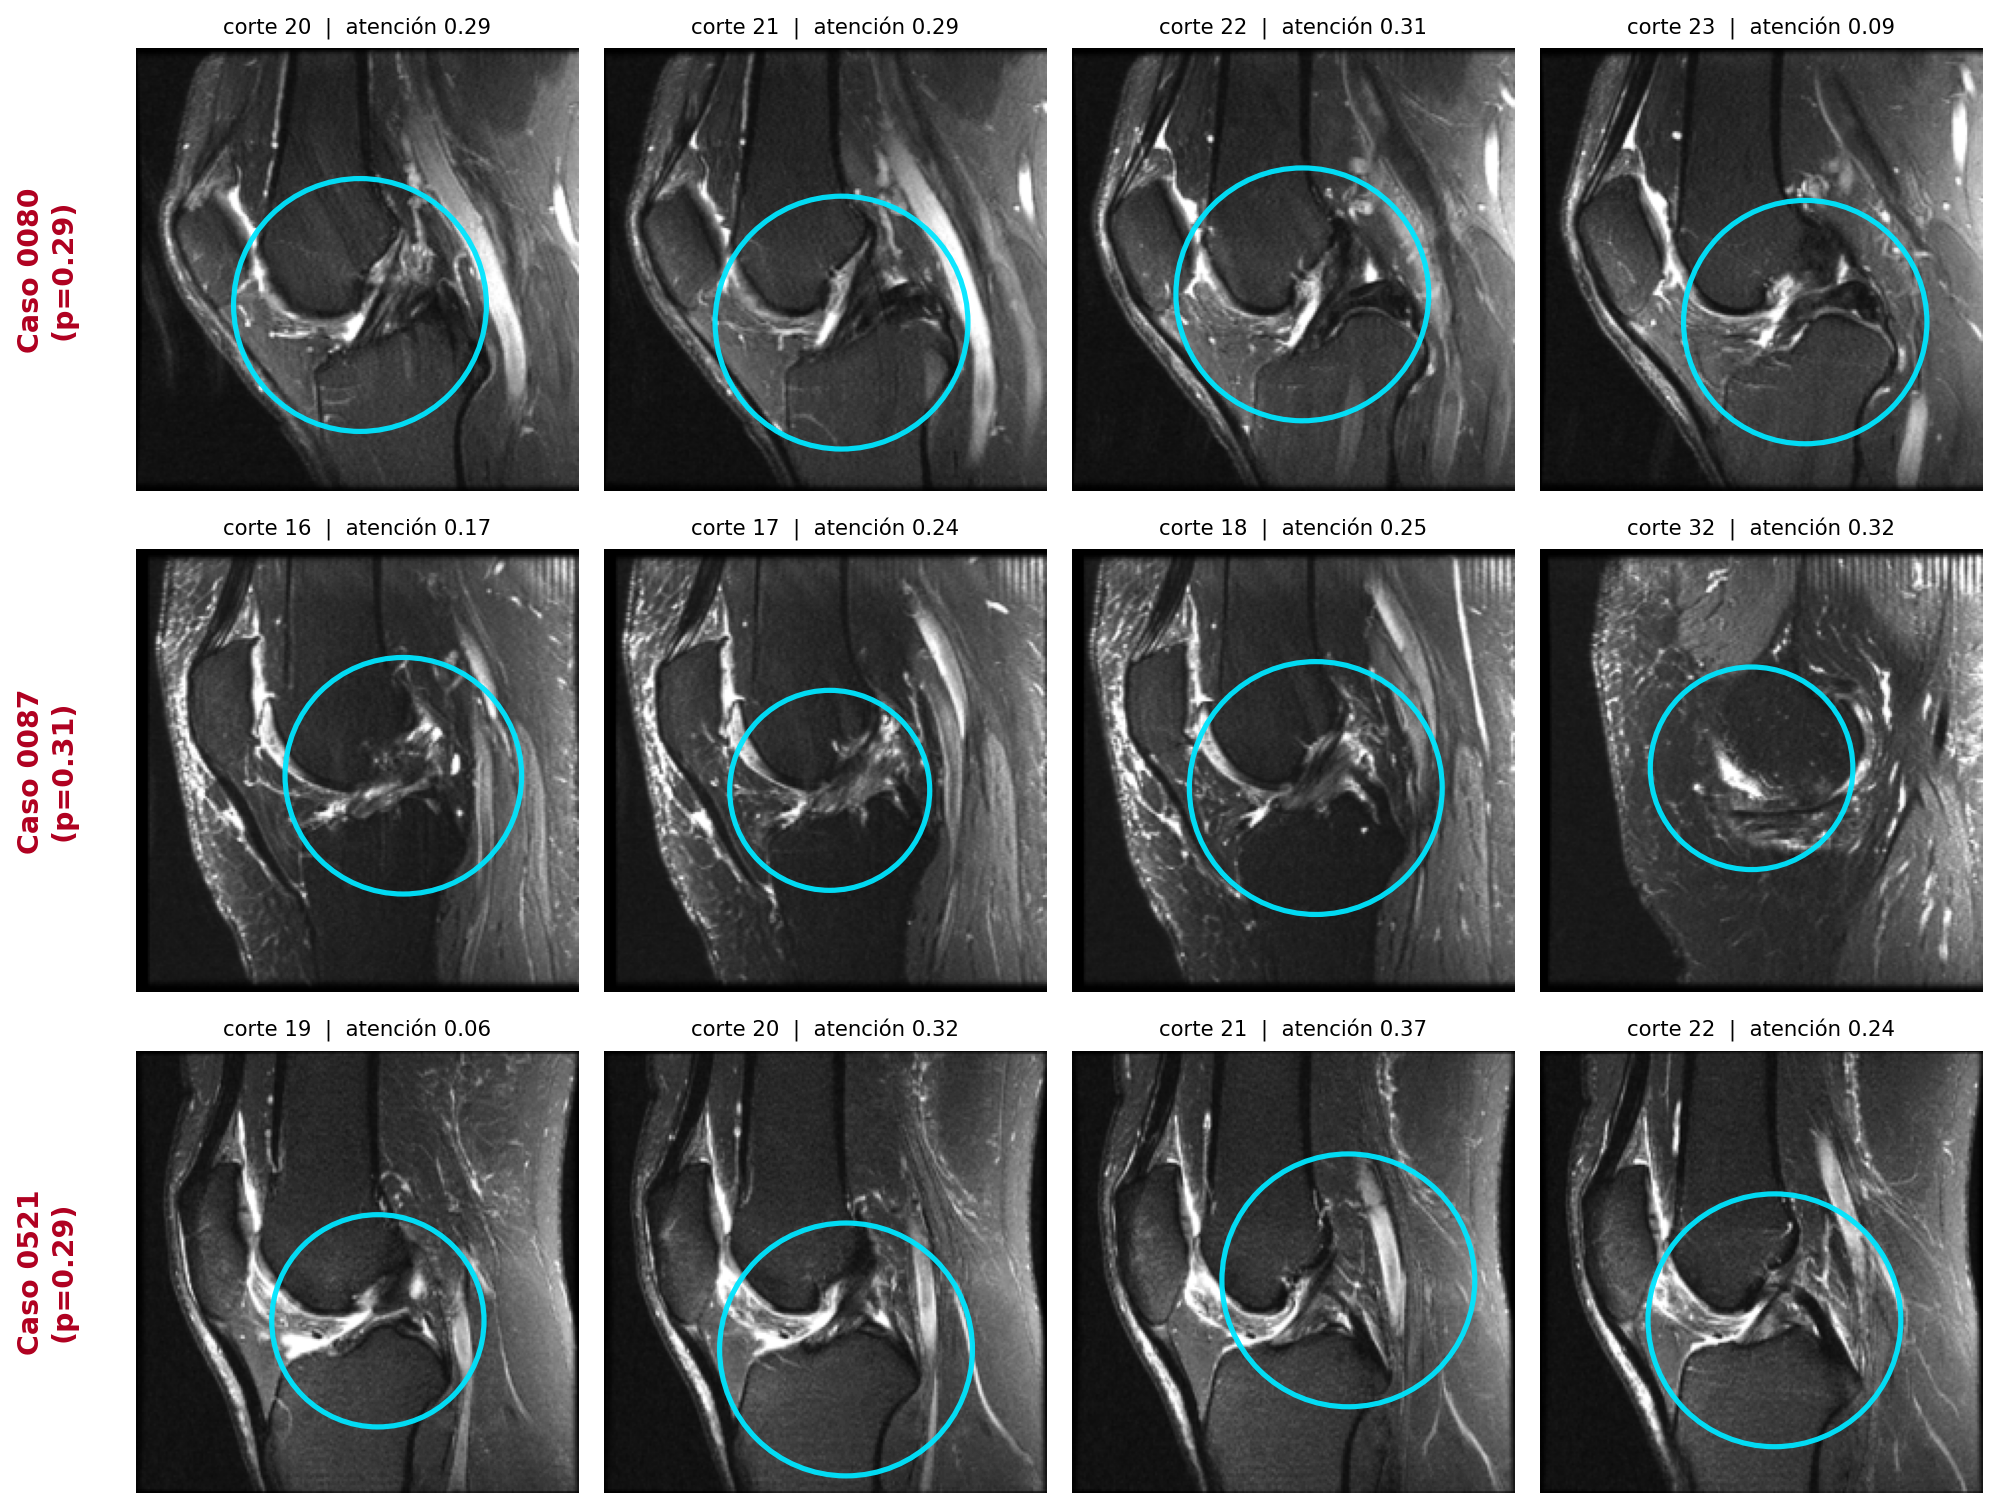
\includegraphics[width=\textwidth]{figs/outputs/fn_comunes_sagital_gradcam.png}
\caption{El círculo señala la zona del ligamento cruzado anterior (escotadura intercondílea) en los cortes sagitales seleccionados de los tres falsos negativos comunes del conjunto de test (casos 0080, 0087 y 0521), dejando visible la anatomía. En los tres estudios la etiqueta real es rotura del LCA.}
\label{fig:fn_comunes}
\end{figure}

% -------------------------------------------------------------------------
% VALIDACION EXTERNA CROACIA
% -------------------------------------------------------------------------

\section{Validación externa}

\subsection{Transferencia directa (zero-shot)}
\label{subsec:validacion_externa_croacia}

La generalización externa se evaluó en el conjunto de Croacia descrito en el capítulo de materiales. La evaluación se realizó en el plano sagital y sin entrenamiento adicional, por lo que corresponde a un escenario \textit{zero-shot}.

Las métricas principales se presentan en la Tabla~\ref{tab:croacia_metricas} y las matrices de confusión correspondientes en la Figura~\ref{fig:croacia_confusion}.

\begin{table}[H]
\centering
\scriptsize
\caption{Validación externa \textit{zero-shot} sobre el test del conjunto de Croacia (sin reajuste de pesos).}
\label{tab:croacia_metricas}
\begin{tabularx}{\textwidth}{
>{\raggedright\arraybackslash}X
>{\centering\arraybackslash}m{1.25cm}
>{\centering\arraybackslash}m{1.25cm}
>{\centering\arraybackslash}m{1.25cm}
>{\centering\arraybackslash}m{1.25cm}
>{\centering\arraybackslash}m{1.25cm}
>{\centering\arraybackslash}m{1.25cm}
}
\toprule
\textbf{Modelo} &
\textbf{AUC} &
\textbf{Acc} &
\textbf{Prec.} &
\textbf{Recall} &
\textbf{Esp.} &
\textbf{F1} \\
\midrule
ResNet50   & 0.7847 & \textbf{0.8702} & \textbf{0.8699} & 0.5595 & \textbf{0.9725} & 0.6810 \\
ViT-Small  & 0.8574 & 0.8451 & 0.6889 & \textbf{0.6828} & 0.8986 & \textbf{0.6858} \\
Swin-Tiny & \textbf{0.8821} & 0.8659 & 0.8377 & 0.5683 & 0.9638 & 0.6772 \\
\bottomrule
\end{tabularx}
\end{table}

\begin{figure}[H]
\centering
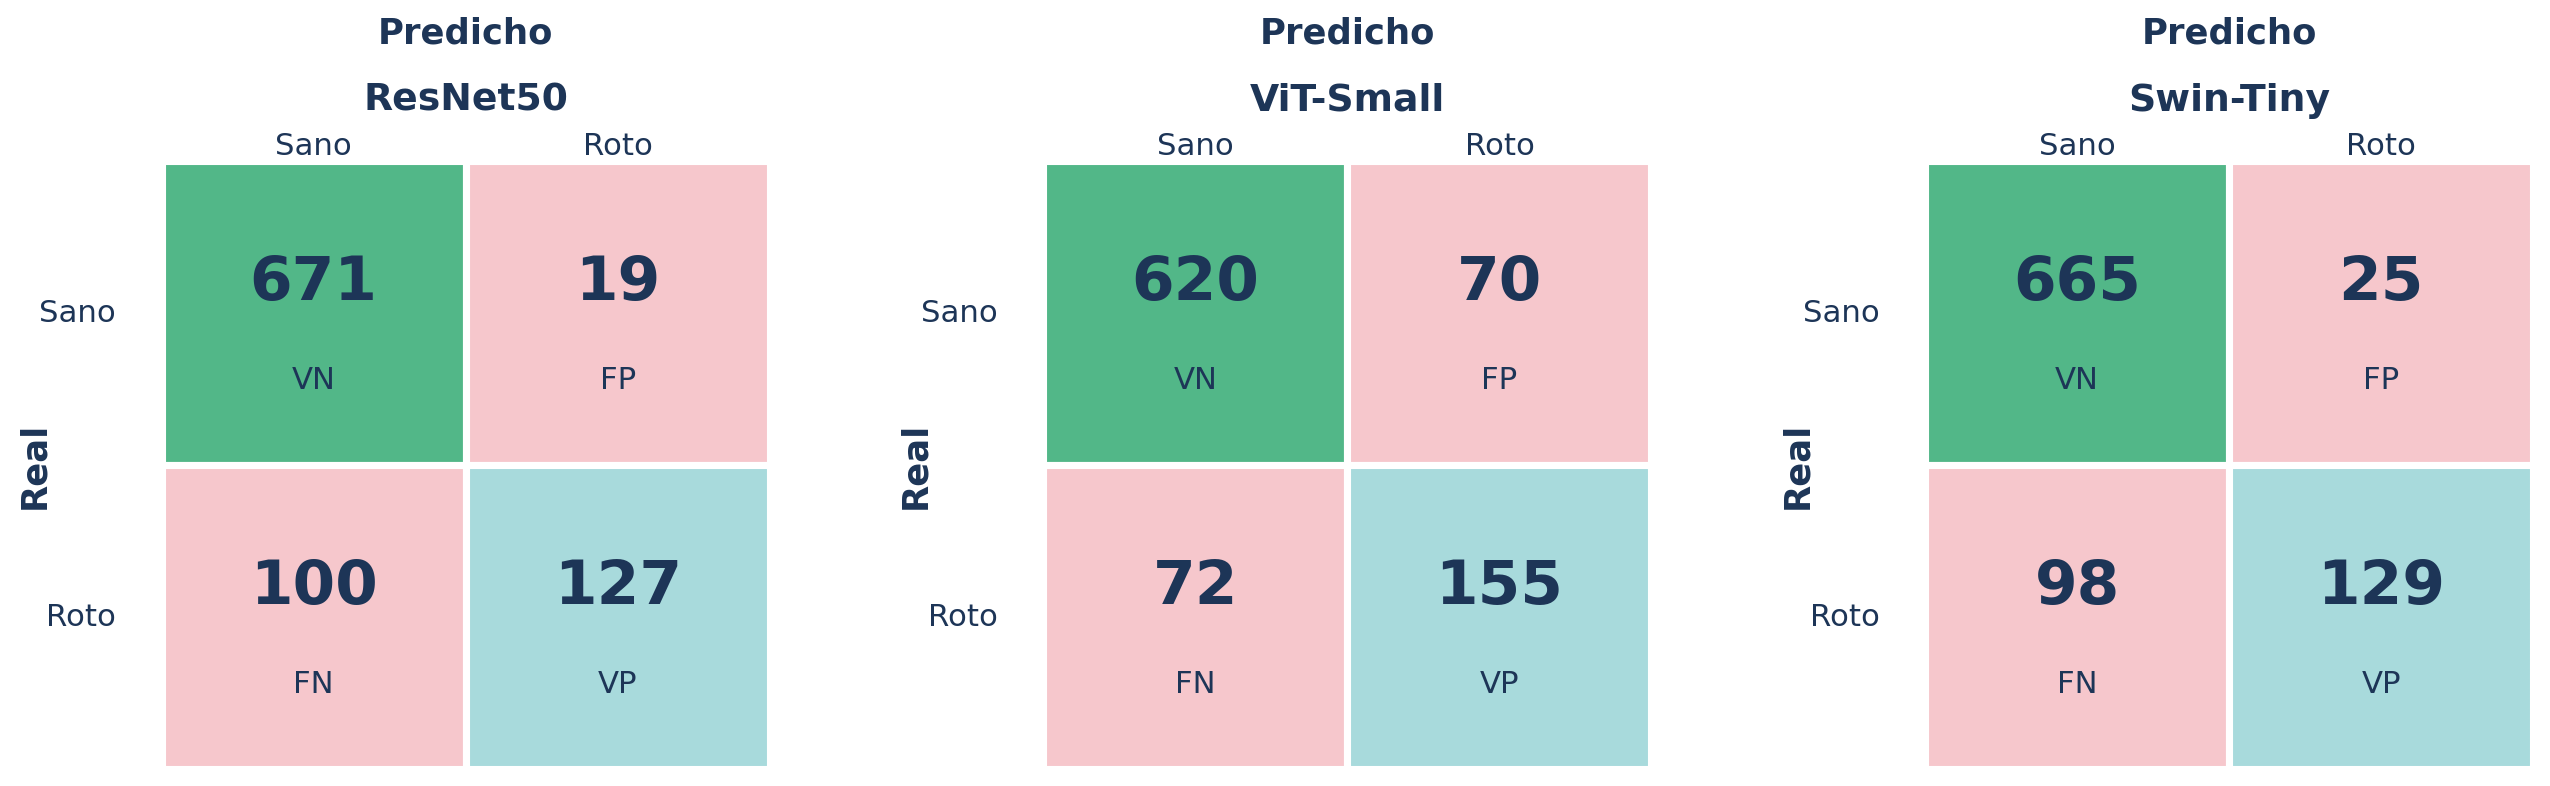
\includegraphics[width=\textwidth]{figs/outputs/CROACIA_cm_grafica.png}
\caption{Matrices de confusión de los tres modelos en la validación externa \textit{zero-shot} (test del conjunto de Croacia, plano sagital, sin reajuste de pesos). VN: verdadero negativo; FP: falso positivo; FN: falso negativo; VP: verdadero positivo.}
\label{fig:croacia_confusion}
\end{figure}

Los resultados evidencian un cambio de dominio relevante entre MRNet y el conjunto de Croacia. Todos los modelos reducen su sensibilidad en la validación externa, lo que indica que las diferencias de adquisición, población, escáner o protocolo pueden afectar al punto operativo aprendido en el dominio original.

En la evaluación externa, Swin-Tiny obtuvo el mayor AUC, con 0.8821, mientras que ViT-Small alcanzó la mayor sensibilidad, con 0.6828.

% -------------------------------------------------------------------------
% FINE-TUNING CROACIA
% -------------------------------------------------------------------------

\subsection{Adaptación de dominio (fine-tuning)}
\label{subsec:fine_tuning_croacia}

Para analizar la adaptación al nuevo dominio, se realizó \textit{fine-tuning} sobre el conjunto de Croacia.

El modelo utilizado para este experimento fue Swin-Tiny en el plano sagital. La configuración de entrenamiento incluyó una tasa de aprendizaje inicial de $2 \times 10^{-4}$, pérdida BCE con \texttt{pos\_weight} = 3.0314 para compensar el desbalance de clases, \textit{dropout} de 0.3 en la entrada del clasificador y \textit{dropout} de 0.2 en la capa densa final. Durante las dos primeras épocas se mantuvo congelado el \textit{backbone}, entrenando únicamente la cabecera clasificadora. A partir de la tercera época se realizó ajuste completo de los pesos del modelo, con reducción de la tasa de aprendizaje en caso de estancamiento.

Una vez realizada la validación externa \textit{zero-shot} sobre el conjunto completo de Croacia, se creó una partición específica de entrenamiento, validación y prueba para adaptar el modelo al nuevo dominio. El rendimiento antes y después del ajuste se evaluó sobre el subconjunto de prueba de Croacia, no sobre MRNet. Los resultados principales se muestran en la Tabla~\ref{tab:fine_tuning_croacia_test}.

\begin{table}[H]
\centering
\small
\caption{Evaluación del modelo Swin-Tiny sagital sobre el test de Croacia antes y después del fine-tuning.}
\label{tab:fine_tuning_croacia_test}
\begin{tabularx}{\textwidth}{
>{\raggedright\arraybackslash}X
>{\centering\arraybackslash}m{2.2cm}
}
\toprule
\textbf{Evaluación en Croacia test} &
\textbf{AUC} \\
\midrule
Antes del fine-tuning  & 0.9236 \\
Después del fine-tuning & 0.9362 \\
Diferencia & +0.0126 \\
\bottomrule
\end{tabularx}
\end{table}

Tras el \textit{fine-tuning}, el AUC sobre el test de Croacia aumentó de 0.9236 a 0.9362. Por tanto, el ajuste con datos del nuevo dominio produjo una mejora moderada en la capacidad discriminativa del modelo sagital. Esta comparación debe interpretarse separadamente de la validación \textit{zero-shot} anterior: primero se evaluó la transferencia directa sobre Croacia sin entrenamiento adicional y, posteriormente, se evaluó el efecto de adaptar el modelo utilizando las particiones de entrenamiento y validación de Croacia.

Las curvas asociadas al ajuste fino no se incorporan como figuras principales porque la conclusión relevante queda resumida por la comparación antes/después del AUC. Su función es comprobar la dinámica de entrenamiento y la ausencia de inestabilidades evidentes, por lo que se consideran material complementario.

\subsection{Prueba ilustrativa sobre estudios propios}

Más allá de la evaluación cuantitativa sobre los conjuntos públicos, el sistema se sometió a una prueba cualitativa adicional sobre estudios de resonancia magnética de rodilla de adquisición propia, completamente ajenos a los datos empleados durante el desarrollo. En esta prueba informal, el sistema produjo predicciones coherentes con el estado real de las articulaciones analizadas. Aunque por su carácter anecdótico y su tamaño muestral no constituye una validación estadística, este ensayo resulta ilustrativo de la aplicabilidad del sistema sobre datos completamente nuevos y refuerza, desde un punto de vista cualitativo, la robustez observada en la validación externa.

% -------------------------------------------------------------------------
% EFECTO DEL TAMAÑO DEL MODELO
% -------------------------------------------------------------------------

\section{Efecto del tamaño del modelo}
\label{subsec:efecto_tamano}

Una decisión metodológica relevante de este trabajo es el uso de arquitecturas compactas (del orden de 22 a 28 millones de parámetros) en lugar de sus variantes mayores. Para justificarla se entrenaron, bajo el mismo protocolo multi-semilla y el mismo \textit{pipeline}, las variantes de mayor capacidad de cada familia de transformers y se compararon con las versiones compactas empleadas como modelos principales. La Tabla~\ref{tab:efecto_tamano} resume el resultado.

\begin{table}[H]
\centering
\small
\caption{Efecto del tamaño del modelo dentro de cada familia de transformers (ensamble multi-vista, AUC de test en MRNet).}
\label{tab:efecto_tamano}
\begin{tabularx}{\textwidth}{
>{\raggedright\arraybackslash}X
>{\raggedright\arraybackslash}m{3.0cm}
>{\centering\arraybackslash}m{2.2cm}
>{\centering\arraybackslash}m{2.2cm}
}
\toprule
\textbf{Familia} &
\textbf{Variante} &
\textbf{Parámetros} &
\textbf{AUC test} \\
\midrule
ViT  & ViT-Small (principal) & 22 M & \textbf{0.9433} \\
ViT  & ViT-Base              & 86 M & 0.9364 \\
\midrule
Swin & Swin-Tiny (principal) & 28 M & \textbf{0.9536} \\
Swin & Swin-Small            & 49 M & No converge \\
\bottomrule
\end{tabularx}
\end{table}

En la familia ViT, la variante \textit{Small} (22 M) iguala a \textit{Base} (86 M) en validación (AUC de 0.9837 frente a 0.9834) y la supera ligeramente en test (0.9433 frente a 0.9364), pese a contar con una cuarta parte de los parámetros. En la familia Swin, la variante \textit{Tiny} (28 M) alcanza un AUC de test de 0.9536, mientras que la variante \textit{Small} auténtica (49 M) no llegó a converger de forma estable bajo el mismo protocolo: la mayoría de las semillas colapsaron hacia la solución trivial, con un AUC medio de validación cercano al azar.

Estos resultados indican que, en un conjunto de datos de tamaño moderado como MRNet, aumentar la capacidad del modelo no se traduce en una mejora del rendimiento, e incluso puede dificultar la optimización. La explicación es coherente con la literatura: los modelos con más parámetros requieren mayores volúmenes de datos para explotar su capacidad y, en ausencia de ellos, tienden a sobreajustar o a presentar entrenamientos inestables, especialmente en arquitecturas sin un fuerte sesgo inductivo de localidad. Por tanto, el uso de arquitecturas compactas no solo reduce el coste computacional, sino que constituye la elección más adecuada para este problema, lo que respalda la selección de ViT-Small y Swin-Tiny como modelos principales.

% -------------------------------------------------------------------------
% DISCUSION GENERAL
% -------------------------------------------------------------------------

\section{Discusión final}
\label{subsec:discusion_general_resultados}

Los experimentos muestran, en primer lugar, que el análisis multi-semilla es necesario en datasets médicos de tamaño moderado, ya que la inicialización puede afectar al rendimiento final. También confirman la utilidad de integrar información multi-vista: las tres arquitecturas obtuvieron resultados competitivos al combinar las probabilidades de los planos sagital, coronal y axial.

La comparación de ensambles en MRNet no identifica un ganador absoluto. Cada arquitectura mostró compromisos distintos entre AUC, sensibilidad, precisión y especificidad. Dado el coste clínico de los falsos negativos, los modelos con mayor sensibilidad pueden ser especialmente interesantes como herramientas de cribado, aunque un mayor número de falsos positivos obliga a interpretar sus predicciones como apoyo y no como sustituto de la evaluación radiológica.

Un aspecto que merece atención es la robustez del umbral de decisión $\tau^*$. La estrategia adoptada (Ecuación~\ref{eq:threshold_clinico}) prioriza la sensibilidad bajo una precisión mínima del 75\,\%, lo que resulta coherente con un escenario de cribado donde no detectar una rotura es el error más costoso. Sin embargo, al calibrarse sobre un conjunto de validación reducido (188 estudios, 36 con rotura), el punto operativo presenta cierta inestabilidad. Por un lado, al recalcular $\tau^*$ de forma independiente para cada una de las diez semillas, el umbral varía de manera apreciable (desviación típica de entre 0.06 y 0.09, y un rango de hasta 0.27 en ViT-Small). Por otro, la precisión obtenida en validación ($\approx$0.76) no se mantiene en el conjunto de test, donde desciende a valores de entre 0.63 y 0.66 para las tres arquitecturas. Ambas observaciones indican que, aunque el criterio de selección es reproducible y clínicamente justificado, el valor concreto de $\tau^*$ debe interpretarse con cautela y constituye un argumento adicional a favor del análisis multi-semilla y de una calibración específica por dominio.

Finalmente, la validación externa en Croacia evidencia \textit{domain shift}: Swin-Tiny obtuvo el mayor AUC externo, pero la sensibilidad disminuyó respecto al test interno. El \textit{fine-tuning} sobre Croacia mejoró el AUC en el subconjunto de prueba de ese mismo dominio, aunque la calibración del punto operativo sigue siendo un aspecto crítico. En conjunto, los resultados apoyan el uso de ensambles multi-vista y refuerzan la necesidad de validación externa, calibración multi-centro y ajuste de umbrales específicos por dominio clínico.